%! Author = angela
%! Date = 24/01/24
% !TeX root = ../thesis-main.tex

\chapter{Validation}
\label{ch:validation}
This chapter describes the validation process of the new \ac{dsl} implementation and incarnation.
Validating the hypotheses is a fundamental step for the correct evaluation of the work done.
It is divided into testing and performance comparison, which are the two main aspects of this validation process.
By comparing the performance of the new implementation with the original one, it is possible to understand if the
introduction of the new features has led to an improvement in the performance of the system.

\section{Tests}
\label{sec:tests}
The testing phase is instrumental in affirming the integrity and functionality of the \ac{dsl} codebase developed for this thesis.
Tests serve as a critical mechanism for verifying the behaviour of the DSL across various scenarios, detecting potential bugs,
and validating adherence to specifications.

Since the \ac{dsl} is designed to be multiplatform, tests are written to ensure that the codebase is compatible with
different platforms and the results across platforms must be consistent.

To achieve this, Kotlin offers \emph{Multiplatform Extensions}, which allows the testing of the same codebase across
different platforms, such as \emph{JVM}, \emph{JS}, and \emph{Native}, just by adding needed extensions in the \texttt{build.gradle.kts} file.

For the testing phase, all the targets suppored by \ac{kmp} have been used and are the following:
\begin{itemize}
    \item Linux x64 and ARM64;
    \item Windows x64(MinGW);
    \item MacOS x64 and ARM64;
    \item IOS x64 and (simulator) ARM64;
    \item WatchOS x64 and (simulator) ARM64;
    \item TvOS x64 and (simulator) ARM64;
\end{itemize}

They cover the most common platforms and to ensure that the \ac{dsl} is compatible with the most common
devices, such as smartphones, tablets, and wearables.
Test have been implemented using the \emph{Kotest} framework, which is a flexible and comprehensive testing framework for Kotlin
with multiplatform support.

\paragraph{Unit Tests}
Focused on individual units or components within a software system, unit testing serves to validate their functionality
according to requirements.
Typically conducted by developers as the initial testing phase, it involves automation and occurs each time modifications
are made to the source code to prevent disruption of existing features.
These tests are engineered to verify the smallest units of code, such as individual functions or methods, in isolation
from the broader system context.

\paragraph{Integration Tests}
Integration testing is a software testing methodology used to evaluate the functionality of combined units of code.
It serves to expose faults in the interaction between integrated units, ensuring that they function as expected.
This type of testing is particularly useful in the context of the \ac{dsl} as it allows the verification of the correct
interactions of the different parts of the system.

\subsection{Continuous Integration and Deployment}
\label{subsec:continuous-integration-and-deployment}
\ac{cicd} are software development practices that aim to automate and streamline the process of delivering high-quality software.
\ac{ci} is a development practice where developers frequently integrate their code changes into a shared repository.
Each integration triggers an automated build process, during which the code is compiled, tested, and verified against a
set of predefined criteria.

The primary goals of \ac{ci} are to detect integration errors early, ensure that the codebase remains functional,
and promote collaboration among team members.
\ac{ci} key features include:
    i) automated builds, automatically triggered by committed code changes;
    ii) automated testing, run automatically during the build process;
    iii) immediate feedback, provided to developers regarding the status of their code changes, allowing to address issues promptly;
    iv) version control integration, enabling seamless integration with code repositories.

\ac{cd} extends the principles of \ac{ci} by automating the deployment process after successful integration and testing.
It involves automatically deploying validated code changes to production or staging environments, eliminating manual
intervention and reducing the time between code changes and their availability to users.
\ac{cd} helps streamline the release process, reduce deployment errors, and enable rapid and reliable software delivery.
\ac{cd} key features include:
    i) automated deployment, Deployments to production or staging environments are automated, ensuring consistency and reliability;
    ii) continuous monitoring, integrated into CD pipelines to track application performance and detect issues in real-time;
    iii) rollback mechanisms, in case of deployment failures;
    iv) environment provisioning, pipelines often include steps for provisioning and configuring target environments as part of the deployment process.

\section{Alchemist Simulations}
\label{sec:alchemist-simulations}
Another validation process regards the effective functioning of \emph{Collektive Incarnation} for the \emph{Alchemist} simulator.
To see if the new incarnation is working as expected, examples of simulations have been implemented and run
~\footnote{\url{https://github.com/Collektive/collektive-examples}}.

Using the Alchemist Simulator for validation showcases the capability of Collektive: implementing algorithms to specify
system behavior is straightforward, and execution is both swift and dependable.

\paragraph{Neighbour Counter}
The first example is a simple aggregate program in which the devices count the number of neighbours they have (\Cref{lst:neighbour-counter-example}).
The result is a map of the space in which each node has a value that represents the number of neighbours it has.

\begin{lstlisting}[language=kt, caption={Neighbour counter code example}, label={lst:neighbour-counter-example}]
fun Aggregate<Int>.neighborCounter(): Int = neighboringViaExchange(0)
    .hood(0) { acc, _ -> acc + 1 }
\end{lstlisting}

The resultant simulation appears at first empty, because the nodes are coloured with a gradient that goes from white to
blue based on the number of neighbours they have.
Once the simulation starts and the nodes communicate with each other, the space is filled with colours, and the number of
neighbours and connections is visible, as shown in \Cref{fig:neighbour-counter}.
The simulator also gives the opportunity to move the nodes around the environment, and the number of neighbours is updated
in real-time.

\begin{figure}[ht!]
    \centering
    \begin{subfigure}[b]{0.49\textwidth}
        \centering
        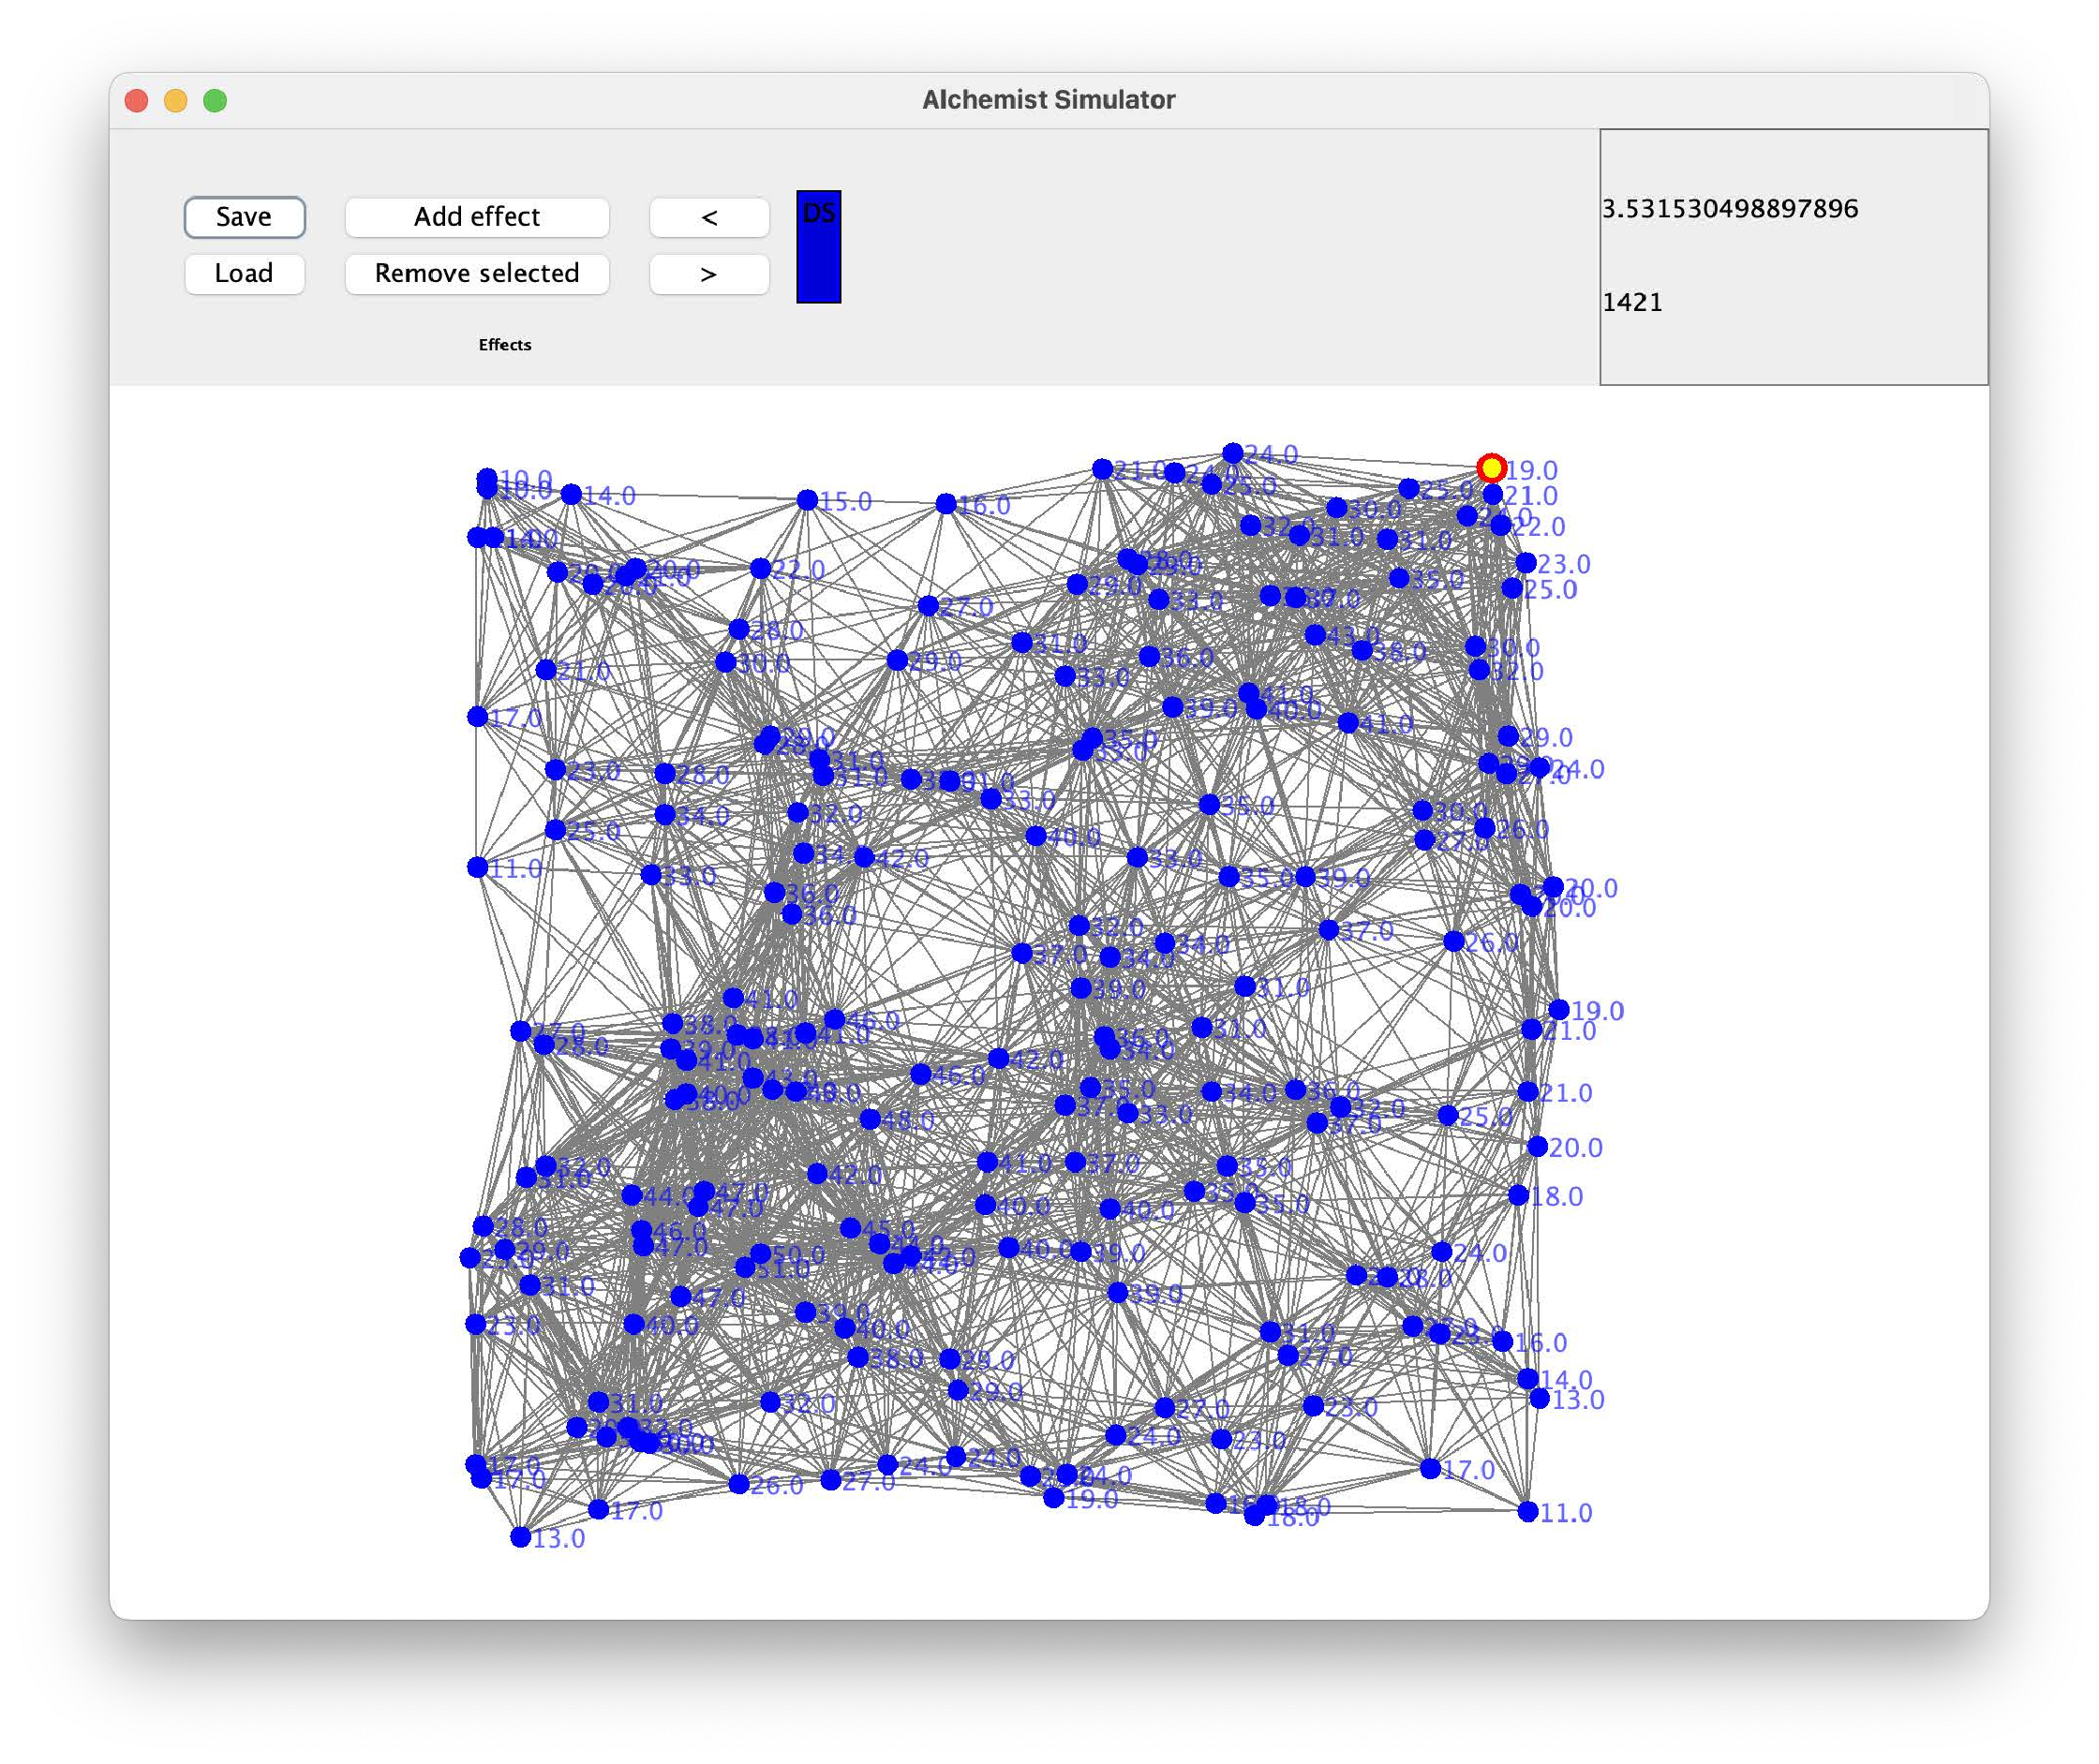
\includegraphics[width=\textwidth]{figures/neighborCounter}
    \end{subfigure}
    \begin{subfigure}[b]{0.49\textwidth}
        \centering
        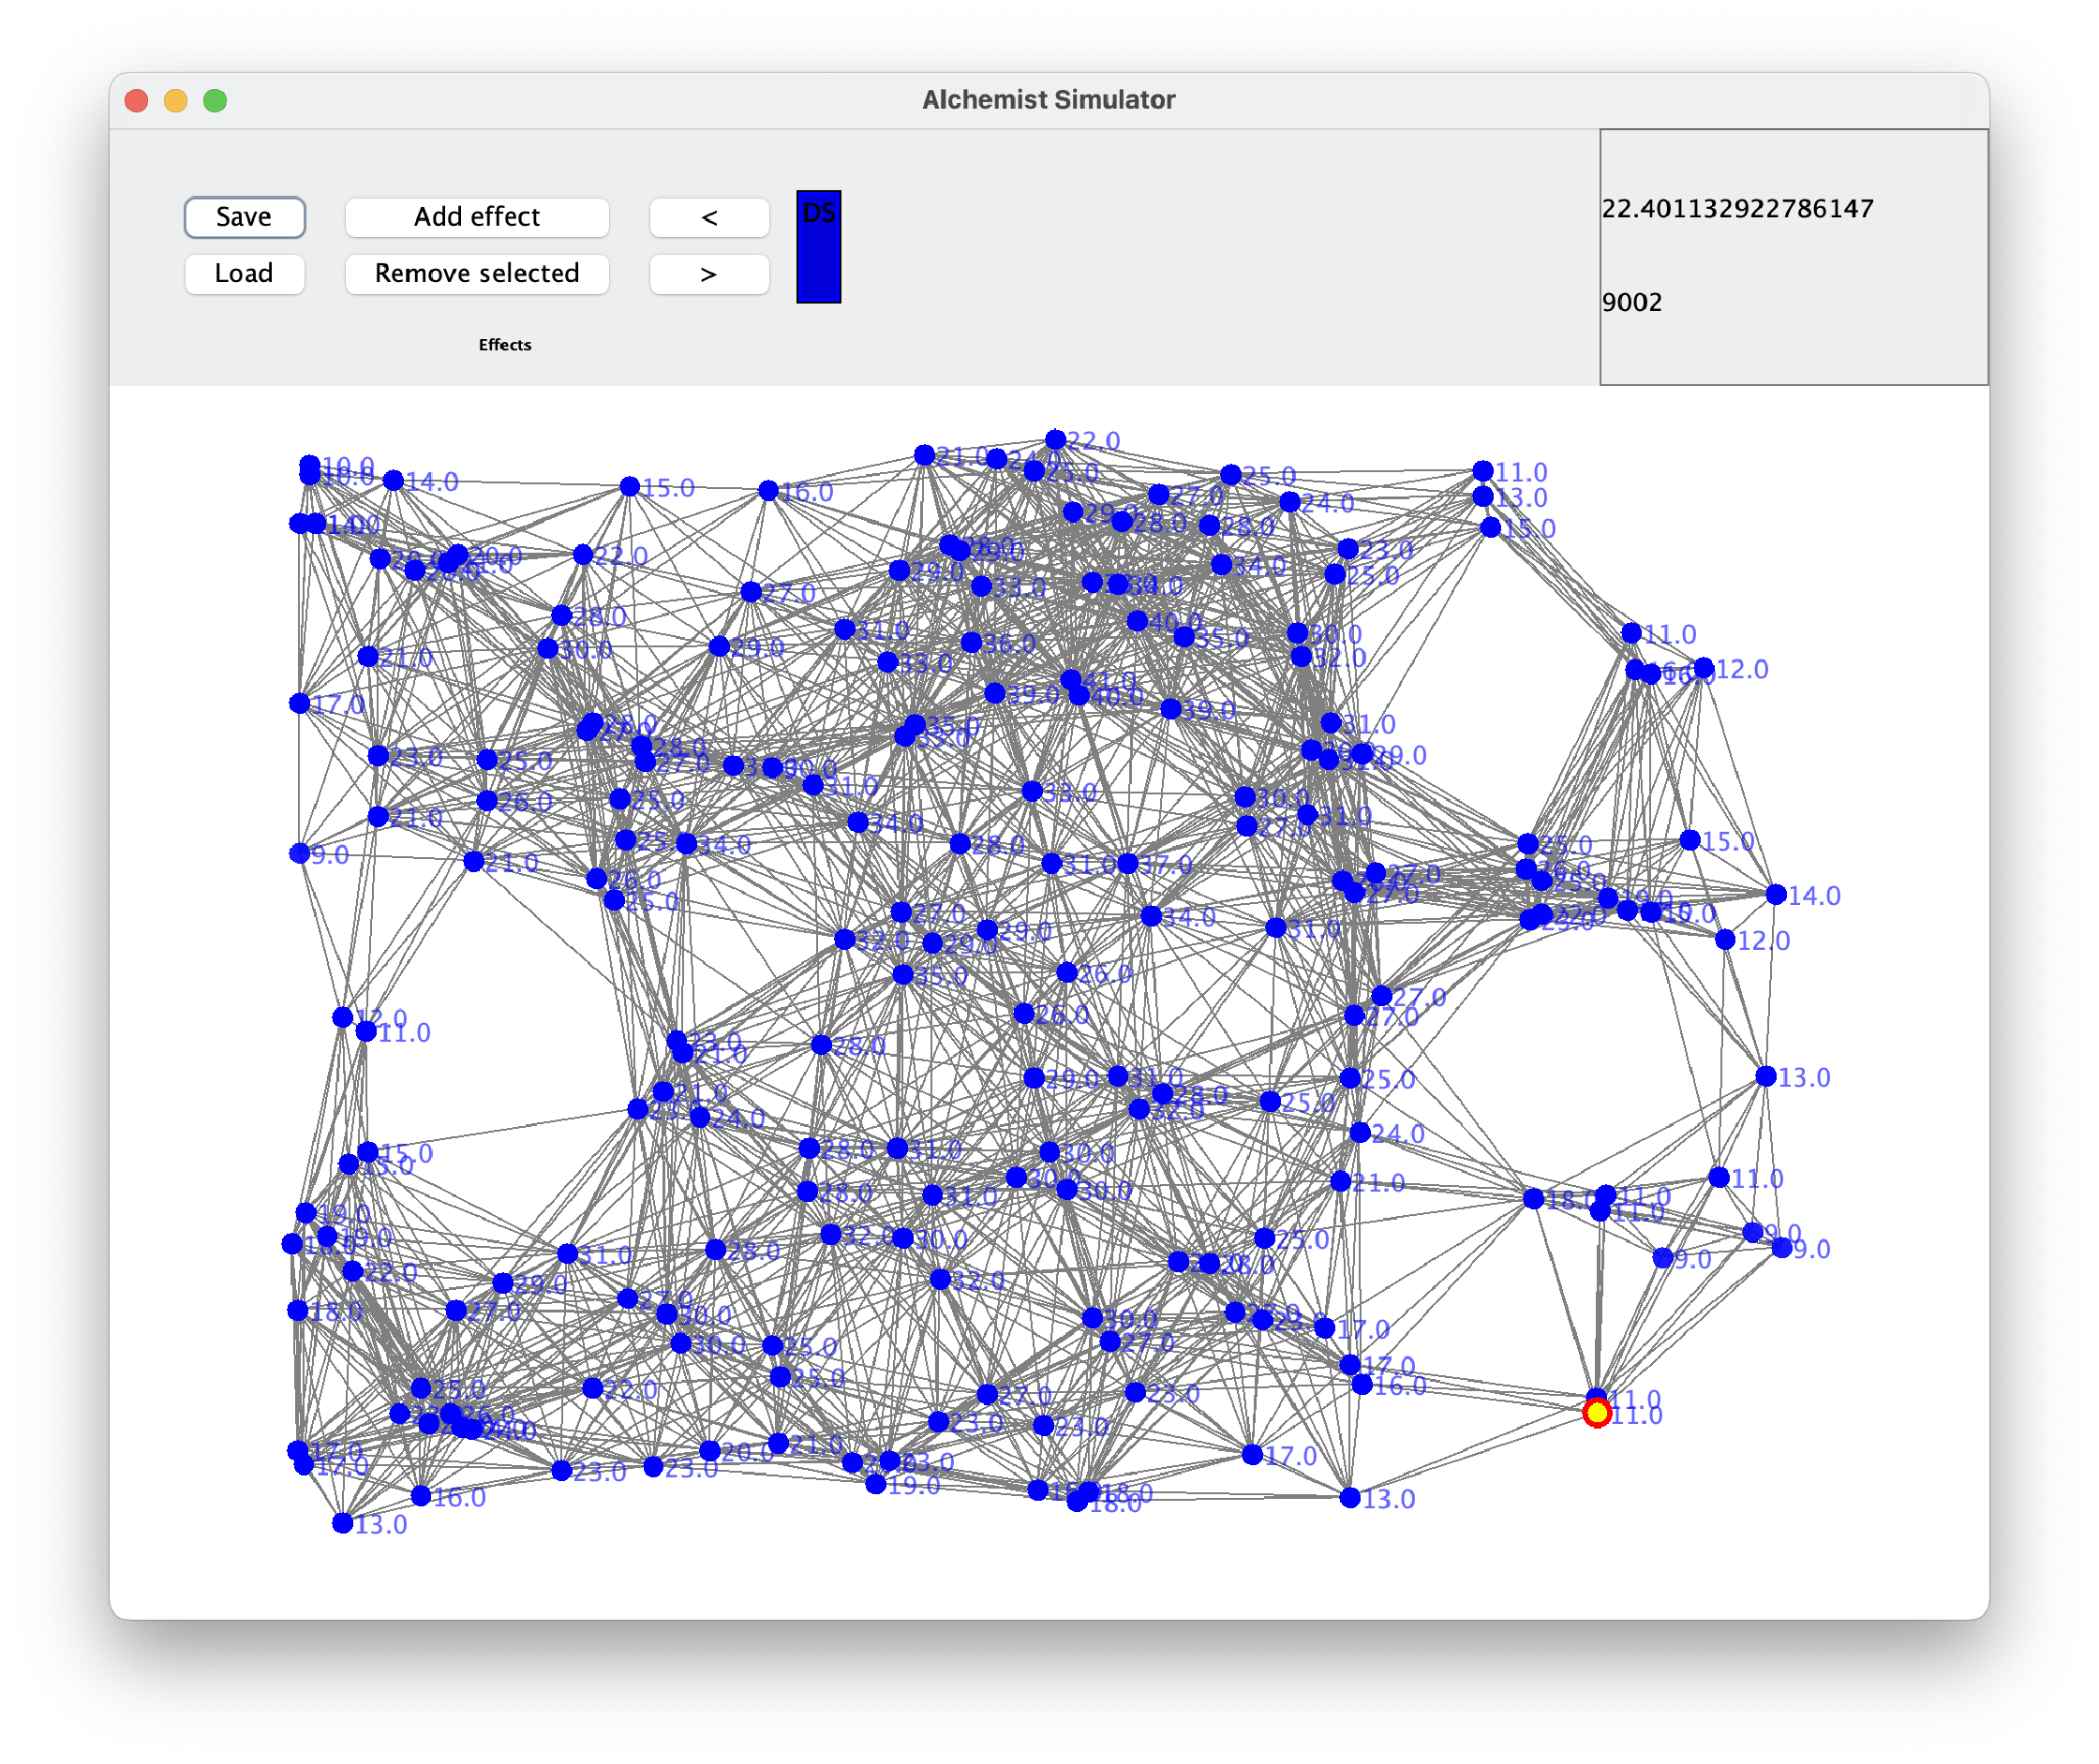
\includegraphics[width=\textwidth]{figures/neighborCounterMoved}
    \end{subfigure}
    \caption{Neighbour counter simulation after some time ad after moving some nodes.}
    \label{fig:neighbour-counter}
\end{figure}

\paragraph{Gradient}
The second example is a simple gradient program in which the devices calculate the distance from a source node and
communicate it to the other nodes (\Cref{lst:gradient-example}).
The result is a map of the space in which each node has a value that represents the distance from the source node,
changing the colour of the nodes based on the distance from the source (seen as a square in \Cref{fig:gradient}).
Also in this case, the simulator gives the opportunity to move the nodes around the environment, and the distance from
the source is updated in real-time.

\begin{lstlisting}[language=kt, caption={Gradient code example}, label={lst:gradient-example}]
context(LocalSensing,DistanceSensor)
fun Aggregate<Int>.gradientEntrypoint(): Double = gradient(sense("source"))

context(DistanceSensor)
fun Aggregate<Int>.gradient(source: Boolean): Double =
    share(POSITIVE_INFINITY) {
        val dist = distances()
        when {
            source -> 0.0
            else -> (it + dist).min(POSITIVE_INFINITY)
        }
    }
\end{lstlisting}

\begin{figure}[ht!]
    \centering
    \begin{subfigure}[b]{0.49\textwidth}
        \centering
        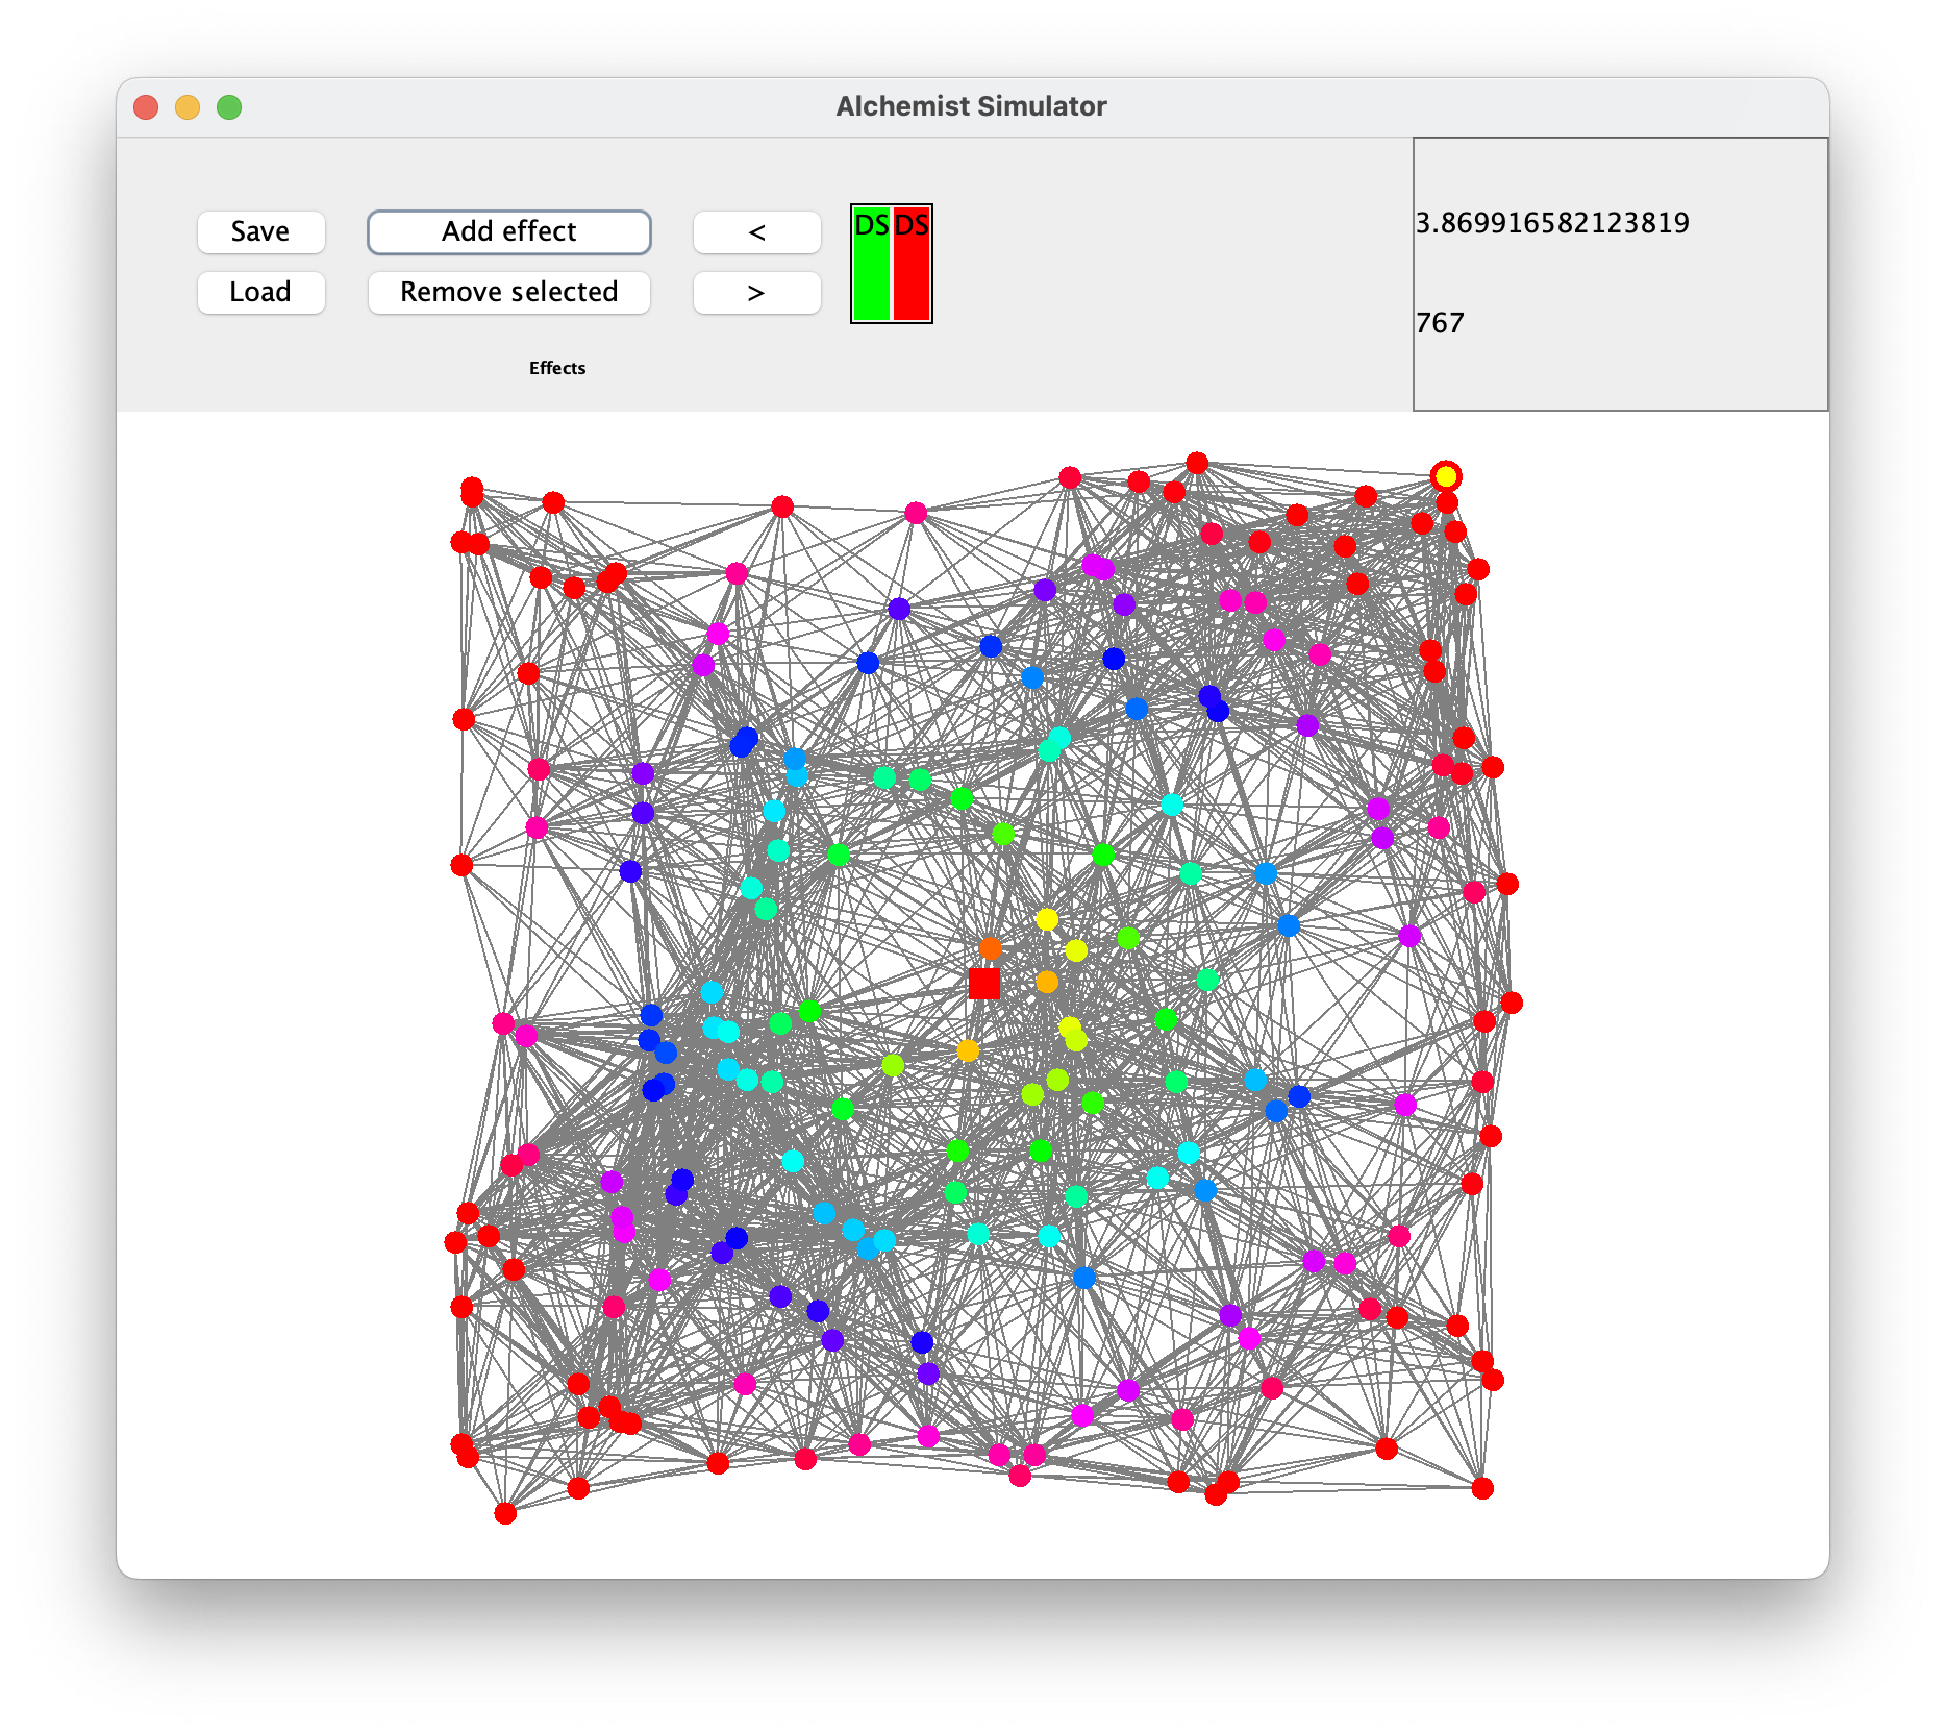
\includegraphics[width=\textwidth]{figures/gradient}
    \end{subfigure}
    \begin{subfigure}[b]{0.49\textwidth}
        \centering
        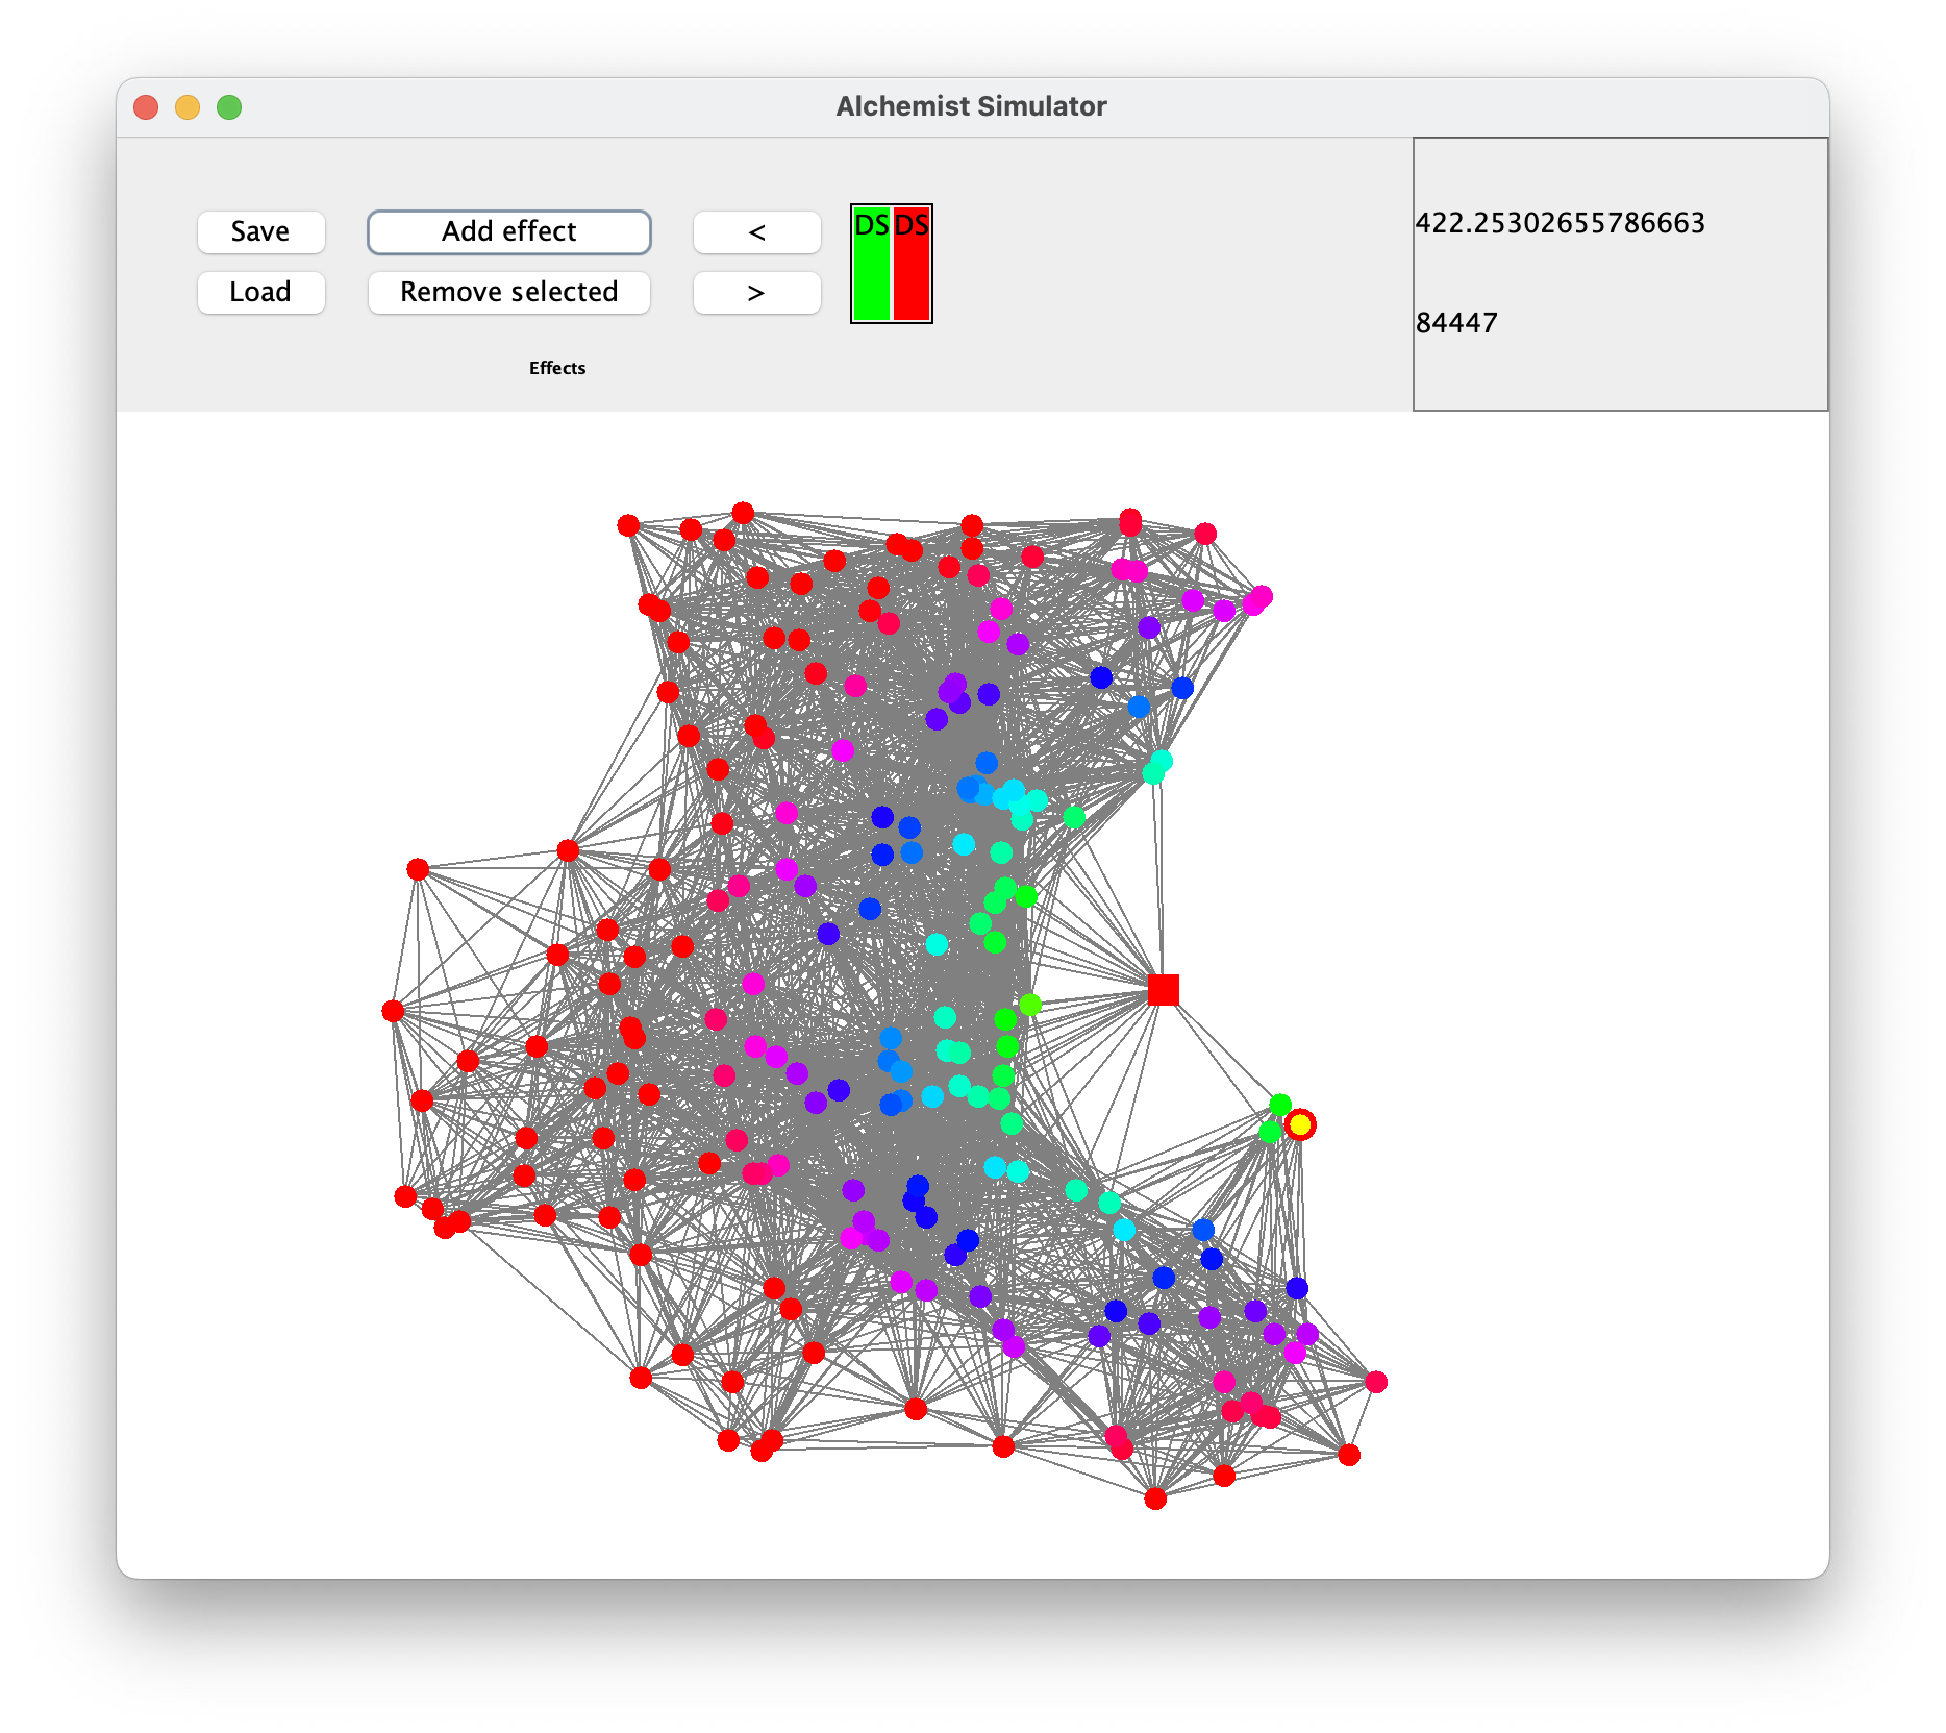
\includegraphics[width=\textwidth]{figures/gradient-moved}
    \end{subfigure}
    \caption{Gradient simulation after some time ad after moving some nodes including the root.}
    \label{fig:gradient}
\end{figure}

\clearpage
\paragraph{Channel with Obstacles}
The third example is a program a bit more complex, recreating a communication pathway (channel) within a distributed
system where data transmission is impeded or affected by various obstacles.
These obstacles could include network congestion, latency, limited bandwidth, or even physical barriers in certain
distributed computing environments.
In the context of aggregate computing, where computations are performed collectively by a network of interconnected
devices or nodes, such obstacles can significantly impact the efficiency and effectiveness of communication and data exchange among the nodes.

From a source node to a target node, the goal is to find a minimum path that avoids obstacles and is the most efficient
in terms of communication letting the information flow through the network (\Cref{lst:channel-with-obstacles-example}).

As shown in \Cref{fig:channel}, the channel (in green) is gradually created from the source (in yellow) towards the
target (in blue), and the obstacles (red) influence the trajectory of the channel, as expected.

\begin{figure}
    \centering
    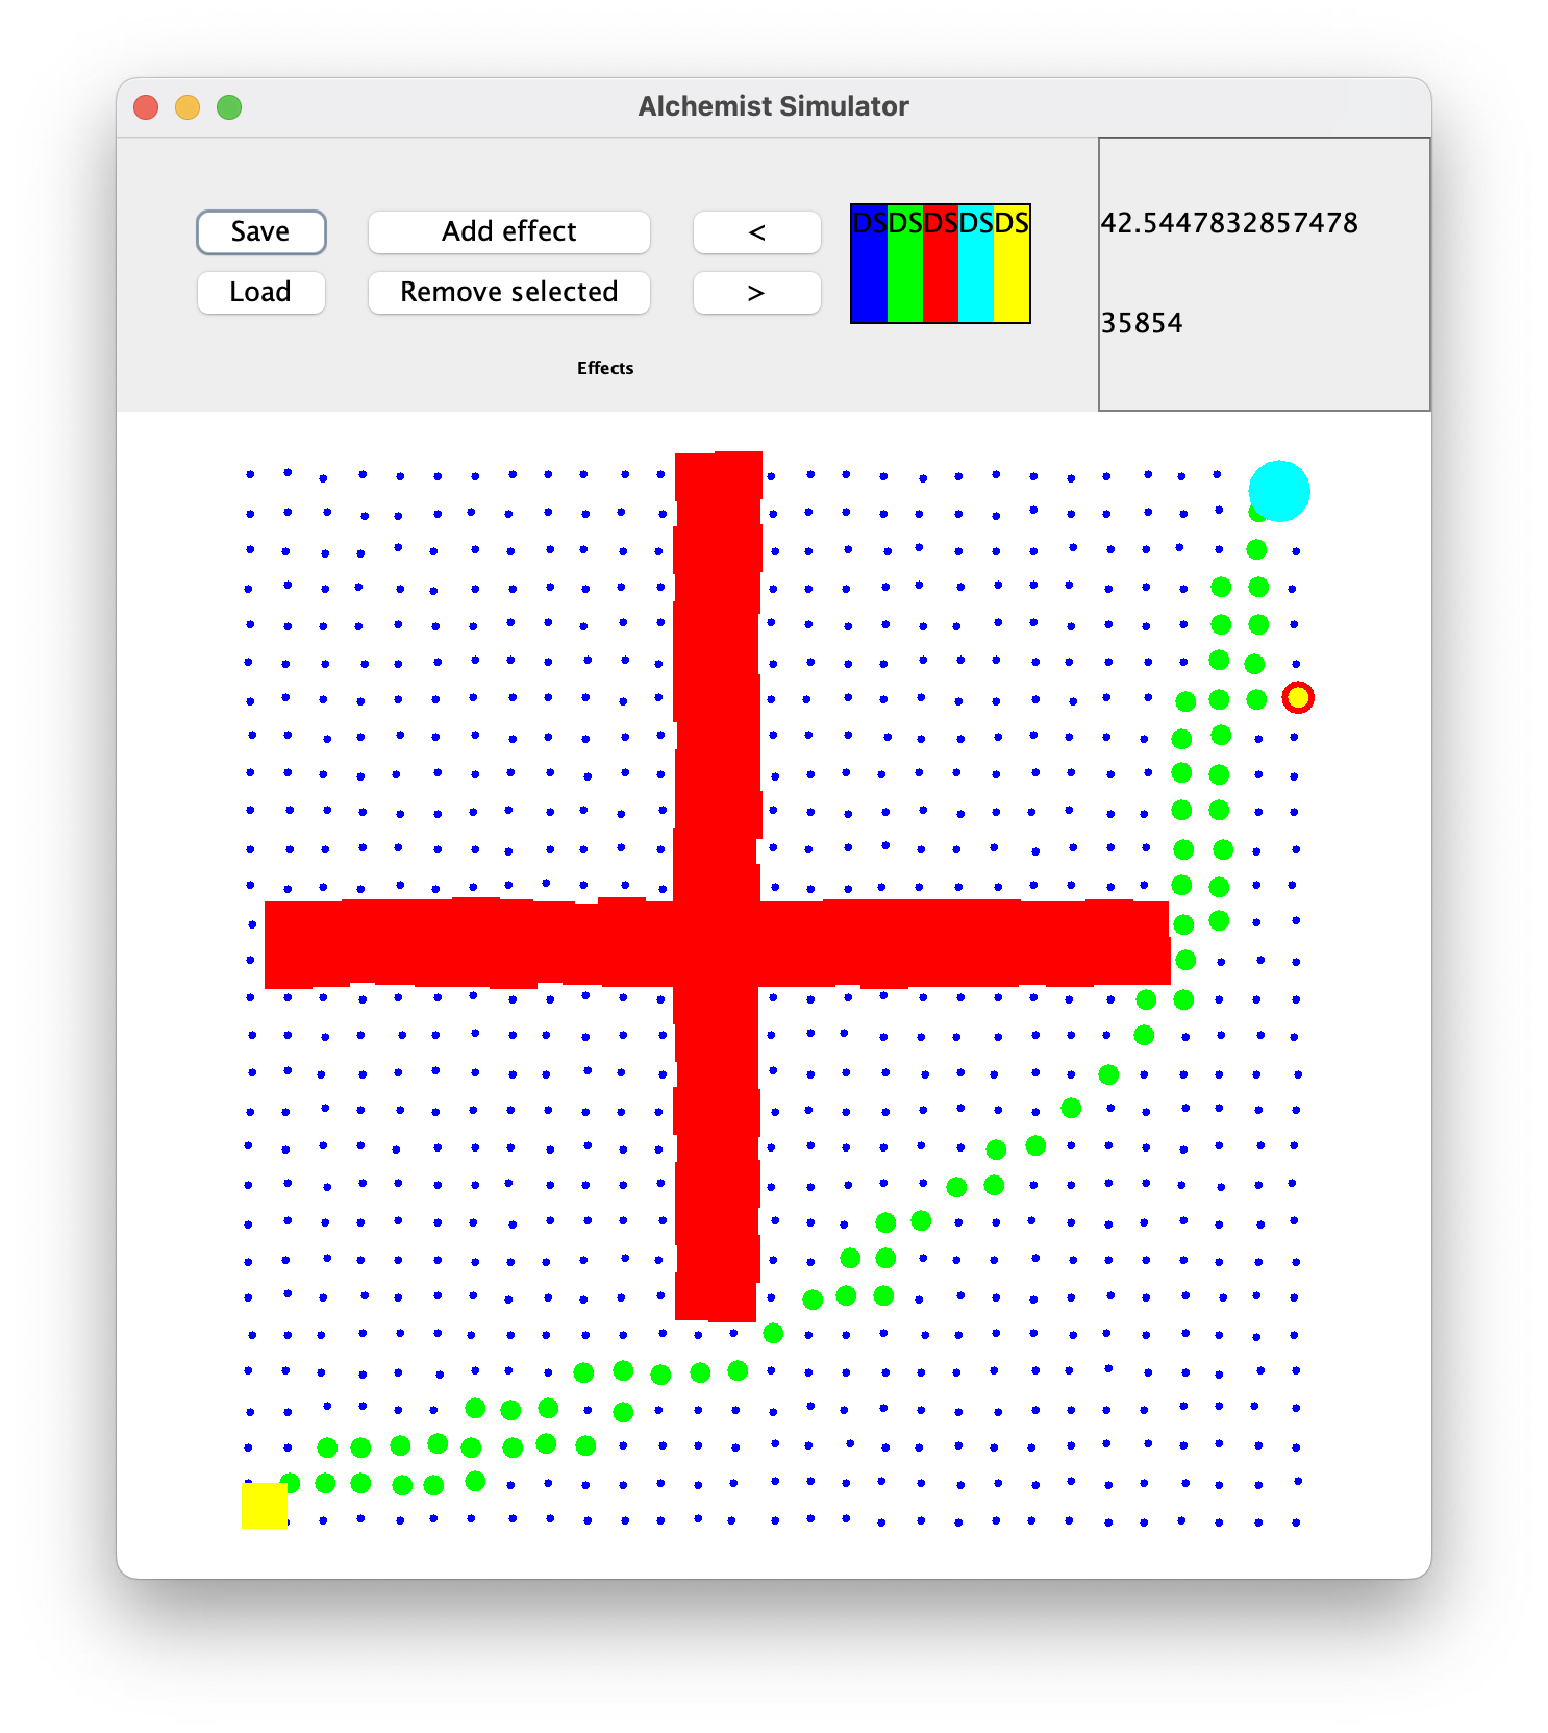
\includegraphics[width=0.6\textwidth]{figures/channel}
    \caption{The resultant simulation of the channel with obstacles.}
    \label{fig:channel}
\end{figure}

\begin{minipage}{\linewidth}
    \begin{lstlisting}[language=kt, caption={Channel with Obstacles code example}, label={lst:channel-with-obstacles-example}]
    context(LocalSensing, DistanceSensor)
    fun Aggregate<Int>.channelWithObstacles(): Boolean =
        if (sense("obstacle")) {
            false
        } else {
            channel(sense("source"), sense("target"), channelWidth = 0.5)
        }

    context(DistanceSensor)
    fun Aggregate<Int>.channel(source: Boolean, target: Boolean, channelWidth: Double): Boolean {
        val sourceDist = gradient(source)
        val targetDist = gradient(target)
        val distBetween = distanceBetween(source, target)
        return !((sourceDist + targetDist).isInfinite() && distBetween.isInfinite()) &&
                sourceDist + targetDist <= distBetween + channelWidth
    }

    context(DistanceSensor)
    fun Aggregate<Int>.distanceBetween(source: Boolean, target: Boolean): Double = broadcast(source, gradient(target))

    context(DistanceSensor)
    fun Aggregate<Int>.broadcast(source: Boolean, value: Double): Double = gradientCast(source, value) { it }

    context(DistanceSensor)
    fun Aggregate<Int>.gradientCast(source: Boolean, initial: Double, accumulate: (Double) -> Double): Double =
        share(POSITIVE_INFINITY to initial) { field ->
            val dist = distances()
            when {
                source -> 0.0 to initial
                else -> {
                    val resultField = dist.alignedMap(field) { distField, (currentDist, value) ->
                        distField + currentDist to accumulate(value)
                    }
                    resultField.fold(POSITIVE_INFINITY to POSITIVE_INFINITY) { acc, value ->
                        if (value.first < acc.first) value else acc
                    }
                }
            }
        }.second
    \end{lstlisting}
\end{minipage}

\section{Performance evaluation}
\label{sec:performance-evaluation}
To have a clear understanding of the performances of the new implementation, it is necessary to compare it with the
\emph{ScaFi} and \emph{Protelis}' incarnations.

It is important to note that the performance discussed evaluates the execution speed of the language together with
the relative incarnation.
It is therefore possible that the competitors may have more performant results with a better implementation of the incarnation.
In more complex experiments, the real effort falls on the language and the management of the fields, and not only on the incarnation.

The comparison is made by running the same simulations on each incarnation and comparing the results.
The simulations~\footnote{\url{https://github.com/angelacorte/collektive-benchmark}} are run on the same machine to
ensure that the comparison is fair, and that the differences are due to the implementation and not to the hardware.

The choice of scenarios for evaluating the performance of the new language in aggregate computing was based on several
factors, each addressing different aspects of the language's capabilities and potential use cases.
Here's a breakdown of the scenarios and the reasons for their selection::
\begin{enumerate}
    \item Simple \textbf{state change}, involves simulating the dynamic evolution of device states over time intervals
        using the \texttt{repeat} construct.
        It was chosen to evaluate the language's efficiency in handling basic state changes, which are fundamental
        operations in aggregate computing systems;
    \item A \textbf{counter of the neighbours}, implemented using the \texttt{neighbouring} construct, it allows for the
        effective calculation of spatial structures.
        This scenario was chosen to evaluate the language's ability to handle computations influenced by the density
        of the network, which affects the number of values present in a field and consequently the amount of computations
        that a device has to perform.
        Assessing the language's performance in handling computations based on network density provides valuable insights into
        its efficiency in dynamically changing environments.
    \item Simple \textbf{branching} operations, included to evaluate the language's performance in handling conditional execution paths.
        Since branching can be resource-intensive, this scenario helps assess the efficiency of the language in managing
        multiple execution paths.
    \item A \textbf{gradient}, which is a particular case of space-time variation implemented using the \texttt{share}
        construct, to associate each device in the system with its shortest distance to the nearest source.
        This algorithm is important because it is a fundamental building block for many other algorithms;
    \item A \textbf{channel with obstacles}, involving computing a path between two points in a network, in this case a
        \textbf{source} and a \textbf{target}, avoiding obstacles and adapting to changes in network topology.
        It was chosen to evaluate the language's ability to handle dynamic network conditions and robustly adapt to
        changes, reflecting real-world scenarios where resilience and adaptability are crucial.
\end{enumerate}

Overall, these scenarios collectively provide a comprehensive assessment of the new language's performance in various aspects
relevant to aggregate computing, including state management, spatial computations, conditional branching, algorithmic
building blocks, and adaptability to dynamic environments.

The first type of test is not influenced by the network density, as each node performs the operation on itself,
independently of the number of neighbours, and there is no exchange of information between the nodes.
In the other types of tests, the density of the network influences the computation, as the number of neighbours of a node
affects the number of values present in a field and consequently the amount of computations that a device has to perform.
Assessing the language's performance in handling computations based on network density provides valuable insights into
its efficiency in dynamically changing environments.

\paragraph{Benchmark set up}
To evaluate the performance of the new language, a set of benchmarks has been designed to compare the performance of the
new language with the existing ones.
The tests have been run with the same parameters in the three different incarnations \emph{Collektive}, \emph{Protelis}, and \emph{ScaFi},
within the \emph{Alchemist} simulator.
Each pair test-incarnation has been run ten times.
The simulations have been performed on a network of medium density (around 30--40 neighbours per node), with a number of
nodes equal to 200 and a communication radius of 7 for the first four types of tests, while for the channel test,
the number of nodes has been increased to 800 and the communication radius to 10, lowering the density of the network to ~10 neighbours per node.
The termination condition of the simulation has been set to 1000 simulated seconds.

The results collected evaluate the execution time of the simulations in milliseconds, and the average execution time of
the ten runs has been calculated.
The results have been analysed and will be further discussed in this section.

\paragraph{Machine Specifications}
The results that will be presented have been obtained by running the simulations on a machine with the following specifications:
\begin{itemize}
    \item \textbf{Processor}: Intel(R) Core(TM) i9-14900KF;
    \item \textbf{RAM}: 64GB 4800mhz;
    \item \textbf{OS}: Linux Manjaro;
\end{itemize}

Additionally, other test runs have been made on a different machine to ensure that the results are consistent across different hardware.

\paragraph{Field Evolution}
The first test has been implemented using the \texttt{repeat} construct, the results of the comparison are shown in \Cref{fig:field-evolution}.

This construct entails a straightforward iteration over its respective field, incrementing the field value with each
iteration for every node within the network.
The \texttt{repeat} construct is used to manage the state of a system by performing state updates or transformations iteratively.
This can be particularly useful in simulations, numerical computations, and real-time systems where state changes occur over time.
Notably, in \emph{Collektive}, this construct operates independently of neighbouring nodes, thereby ensuring enhanced
performance by avoiding information exchange with neighbours.

The program simply increments the value of the field at each iteration; therefore, the results highlight that the difference
of performance may be in the implementation of the field management inside the construct, showing that \emph{Collektive}
is faster than the other languages.

\begin{figure}[ht!]
    \centering
    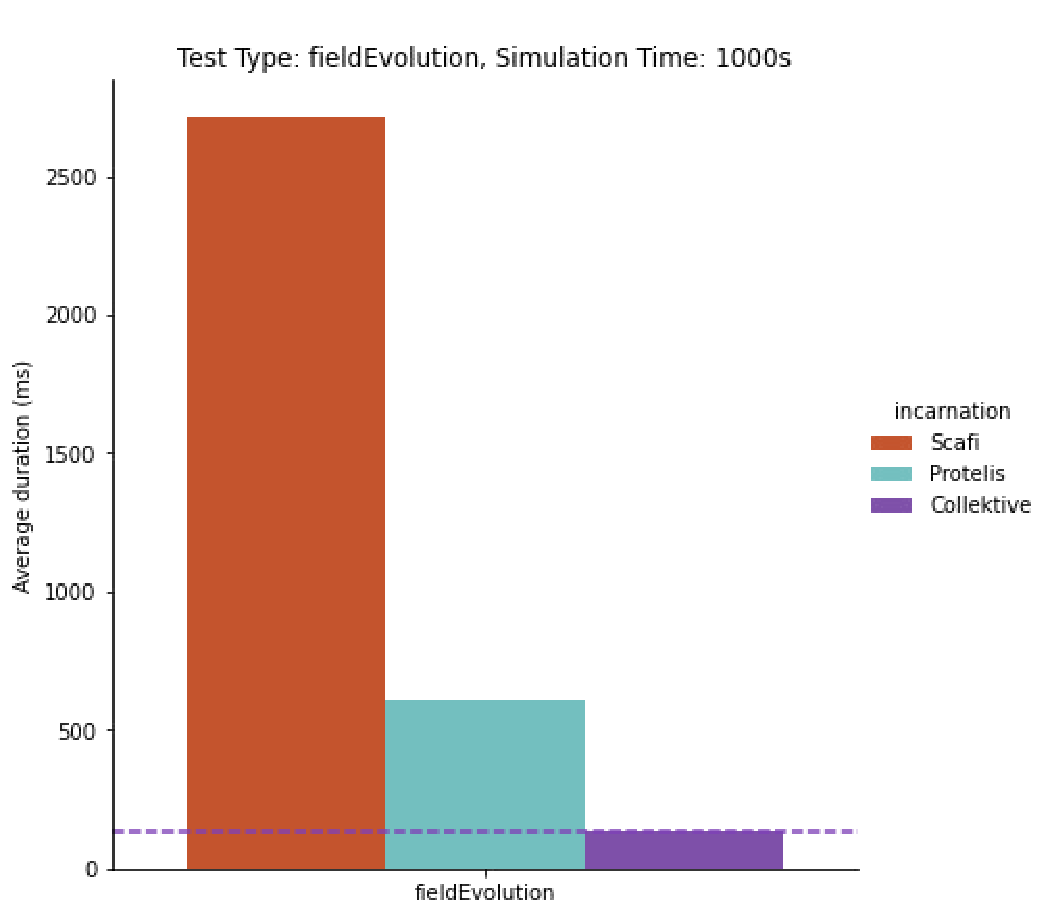
\includegraphics[width=0.6\textwidth]{figures/field-evolution-results}
    \caption{Graph of the results for the field evolution benchmark, showing that on average \emph{Collektive} is $4.51$ times faster
        than \emph{Protelis} and $20.30$ times faster than \emph{ScaFi}.}
    \label{fig:field-evolution}
\end{figure}

\paragraph{Neighbour Counter}
The neighbour counter has been implemented using the \texttt{neighbouringViaExchange} construct, which is used to
manage spatial structures and perform computations based on the information exchanged between the neighbours.
The program is made in such a way to count the number of neighbours each node has, communicating with their neighbours
to exchange information and increment the local value for each neighbour they have.

The network density influences this kind of operation, as the number node's neighbours affects the number of
values present in a field and consequently the number of computations that a device has to perform.
This means that the performances evaluated in this test are affected by the way the language manages the fields and the
messages received from the neighbours.

From the results (\Cref{fig:neghbour-counter}), it can be noticed that the difference with \emph{Protelis} is minimal,
while with \emph{ScaFi} it is significant.
This happens because \emph{Protelis}, being an interpreted language, has advantages in the execution of less complex programs.

\begin{figure}[ht!]
    \centering
    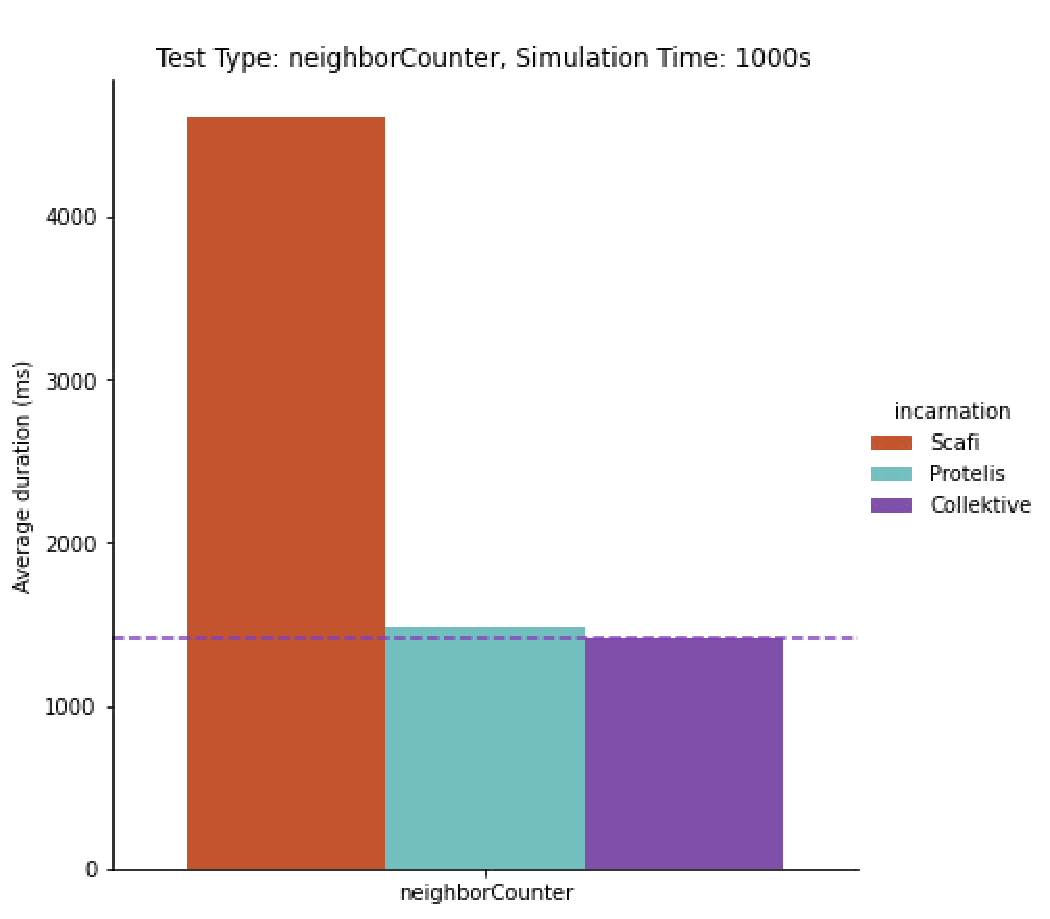
\includegraphics[width=0.6\textwidth]{figures/neighboring-results}
    \caption{Graph of the results for the neighbour-counter benchmark, showing that on average \emph{Collektive} is $1.04$ times faster
    than \emph{Protelis} and $3.25$ times faster than \emph{ScaFi}.}
    \label{fig:neghbour-counter}
\end{figure}

\paragraph{Branching}
``Branching'' happens when a node has to make different evaluations based on a condition (as explained in \Cref{par:conditionals}).
Comparison for this type of test is essential due to the observation that branching operations can be among the most
resource-intensive tasks in terms of execution time, given that they create multiple subprograms and consequently
multiple execution paths to be checked and managed.
In \emph{ScaFi}, branching is handled in a distinct manner, where exceptions are thrown to perform checks on the function to call,
while in \emph{Protelis} and \emph{Collektive}, they follow a more conventional approach, aligning when a function is called.

\begin{lstlisting}[language=kt, caption={Branching code example}, label={lst:branching-example}]
fun Aggregate<Int>.branching() =
    if (sense("source")) {
        neighboringViaExchange(0).hood(0) { acc, _ -> acc + 1 }
    } else {
        0
    }
\end{lstlisting}

As shown in \Cref{lst:branching-example}, the program is made in such a way that if a condition is met, the node
performs a simple neighbouring computation, that is the same as the one in the neighbour counter-test, otherwise it returns a value.

\begin{figure}[ht!]
    \centering
    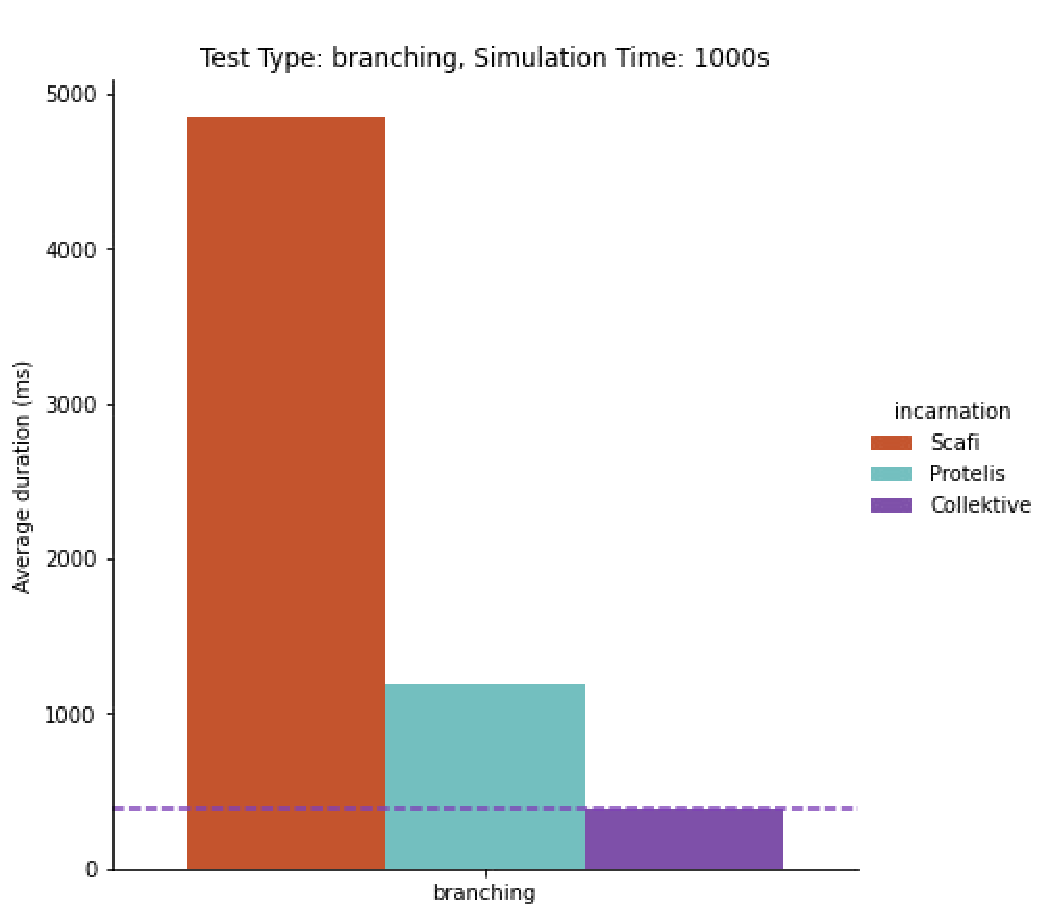
\includegraphics[width=0.6\textwidth]{figures/branching-results}
    \caption{Graph of the results for the branching benchmark, showing that on average \emph{Collektive} is $3.08$ times faster
    than \emph{Protelis} and $12.45$ times faster than \emph{ScaFi}.}
    \label{fig:branching}
\end{figure}

The results depicted in \Cref{fig:branching} illustrate the disparity in performance for this type of operation,
underscoring the benefits of adopting a more traditional alignment approach, rather than the exception-based approach
employed by \emph{ScaFi}.
Note that, being the same implementation as the neighbour counter, the results are influenced in the same way.

\paragraph{Gradient}
The gradient implemented with \emph{Collektive} uses the \texttt{share} construct (based on the \texttt{exchange} construct) to
calculate the distance from a source node and communicate it to the other nodes.
For \emph{Collektive} and \emph{Protelis}, the apparent implementation is the same, while for \emph{ScaFi} is different.
This is because in \emph{ScaFi} the \texttt{gradient} it is not implemented through the \texttt{share} construct, but
it combines \texttt{rep} and \texttt{nbr} to achieve the same result.
Apparently the implementation for \emph{Collektive} and \emph{Protelis} can be the same, but the execution is different, as
\emph{Collektive} leverage on the \texttt{exchange} construct, which manages the fields and the message exchange
in a more efficient way.

\begin{figure}[ht!]
    \centering
    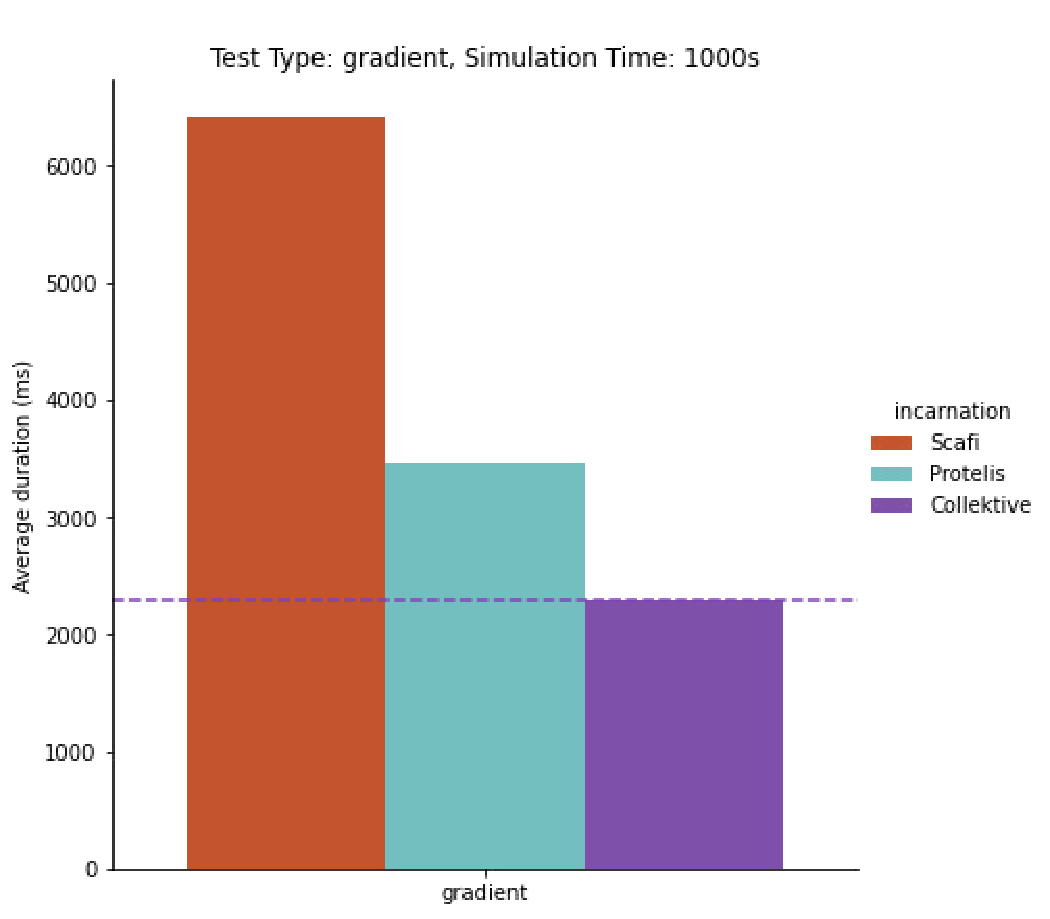
\includegraphics[width=0.6\textwidth]{figures/gradient-results}
    \caption{Graph of the results for the gradient benchmark, showing that on average \emph{Collektive} is $1.51$ times faster
    than \emph{Protelis} and $2.80$ times faster than \emph{ScaFi}.}
    \label{fig:gradient-resutls}
\end{figure}

The results in \Cref{fig:gradient-resutls} show that even with an increase in the amount of communication between nodes,
\emph{Collektive} does not lose performance compared to the other languages.
This demonstrates how the management of the fields and the message exchange are the strength of \emph{Collektive}.

\paragraph{Channel with Obstacles}
Among all the tests, the channel with obstacles is the most complex and the closest to a real-world scenario,
because it simulates challenges encountered in actual deployments.
It involves computing paths while considering obstacles, dynamically adapting to network changes, managing resources
efficiently, and ensuring reliability despite obstacles.
This scenario closely mirrors the complexities of real-world networks, making it a valuable test for evaluating aggregate
computing systems in practical situations.

\begin{figure}[ht!]
    \centering
    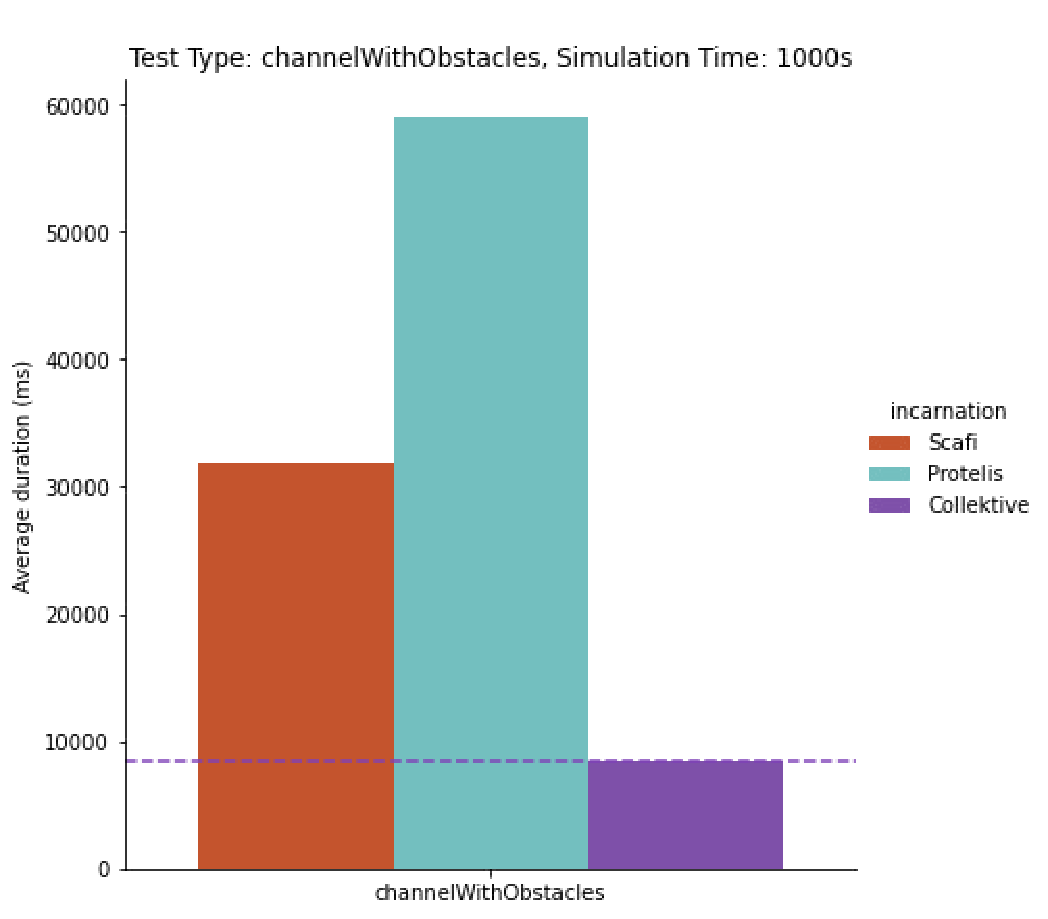
\includegraphics[width=0.6\textwidth]{figures/channel-results}
    \caption{Graph of the results for the channel with obstacles benchmark, showing that on average \emph{Collektive} is $6.91$ times faster
    than \emph{Protelis} and $3.73$ times faster than \emph{ScaFi}.}
    \label{fig:channel-with-obstacles}
\end{figure}

The program is implemented as in \Cref{lst:channel-with-obstacles-example}, so it calculates many times the distances
between nodes, using a bit more complex gradient implementation.
This means that the performance of this test is influenced by the same factors that influence the gradient test.

The results in \Cref{fig:channel-with-obstacles} show that in complex programs, \emph{Protelis} has a significant
disadvantage compared to \emph{Collektive}, while in the other examples they were closer.
This is due to the fact that \emph{Protelis} is an interpreted language and its execution of programs that need to go
deeper in the execution tree is slower.
This test emphasises the strength of \emph{Collektive} in managing fields and message exchange, as the difference in
performance is significant.

\paragraph{Changing the neighbourhood}
Performances may be related to the amount of communication between nodes, meaning that the more communication
between nodes, the more time is spent in the execution of the program.
For this reason, the experiments have been repeated with different network densities to see if the performance changes with
the amount of communication, as the density increases, the number of neighbours a node has increases.
Tests have been performed with low, medium, and high densities.

In the \Cref{fig:speedup}, the speedup of the different incarnations with different network densities on the different tests is shown.
The speedup is calculated as the ratio between the average execution time of the other incarnations and the average execution time of
\emph{Collektive}.
The results show that \emph{Collektive}, even with an increase in the amount of communication between nodes, is still
faster than \emph{Protelis} and \emph{ScaFi}, with a significant difference in the most complex tests.
This is a significant result, as it shows that the language is implemented in such way that can easily handle the increasing
of the fields' size.
This is a fundamental aspect, as the language is designed to be used in real-world scenarios, where the network density
can change over time and can be high.

\begin{figure}[ht!]
    \centering
    \begin{subfigure}[b]{0.49\textwidth}
        \centering
        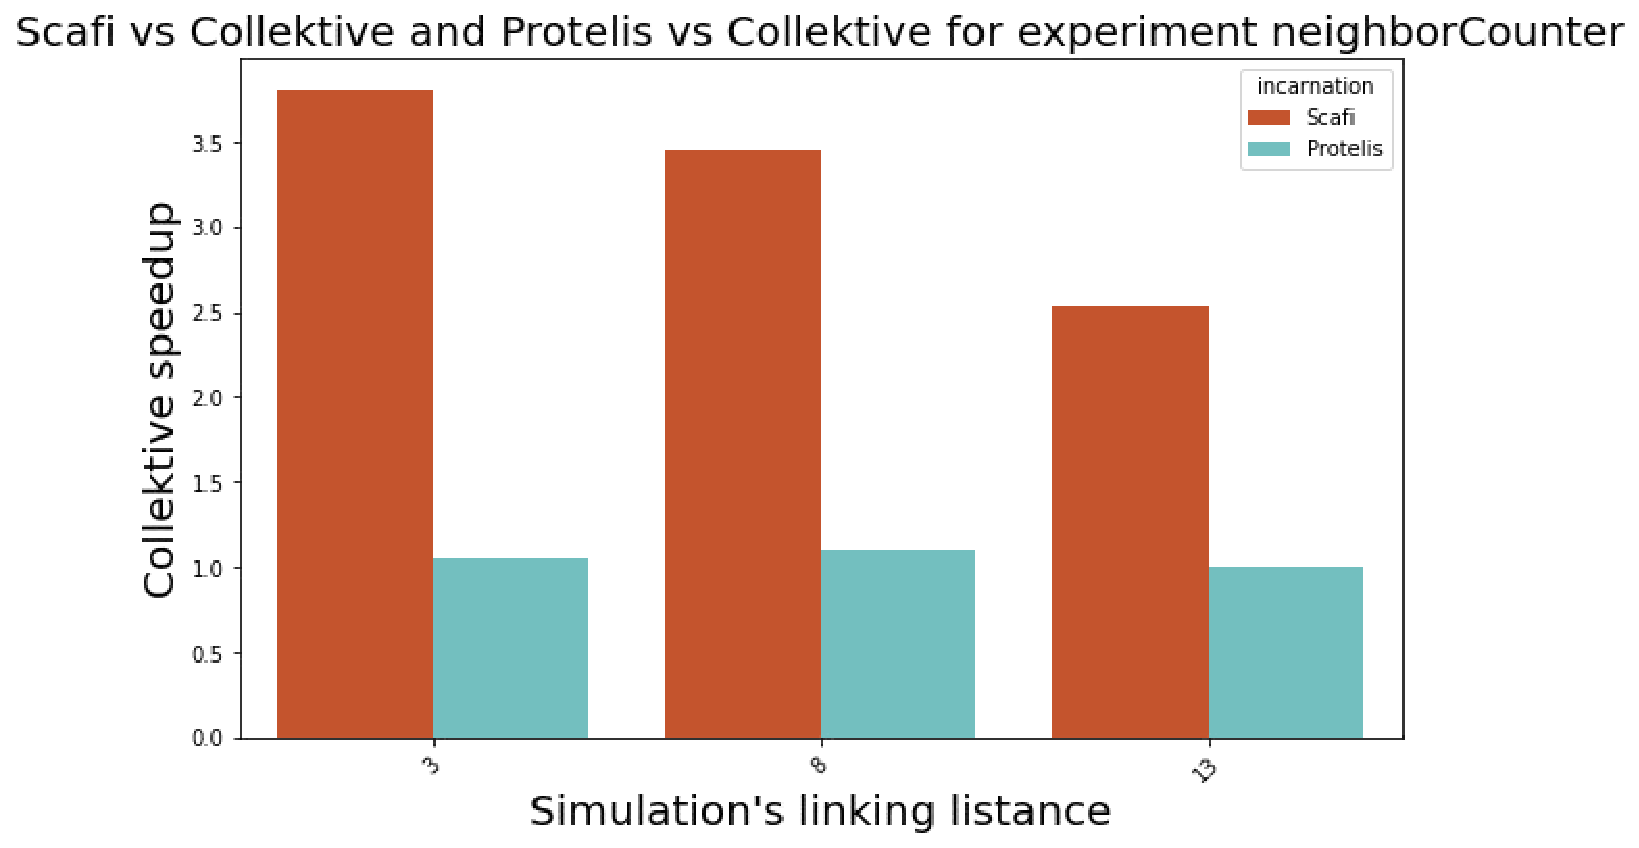
\includegraphics[width=\textwidth]{figures/neighbor-speedup}
    \end{subfigure}
%    \begin{subfigure}[b]{0.49\textwidth}
%        \centering
%        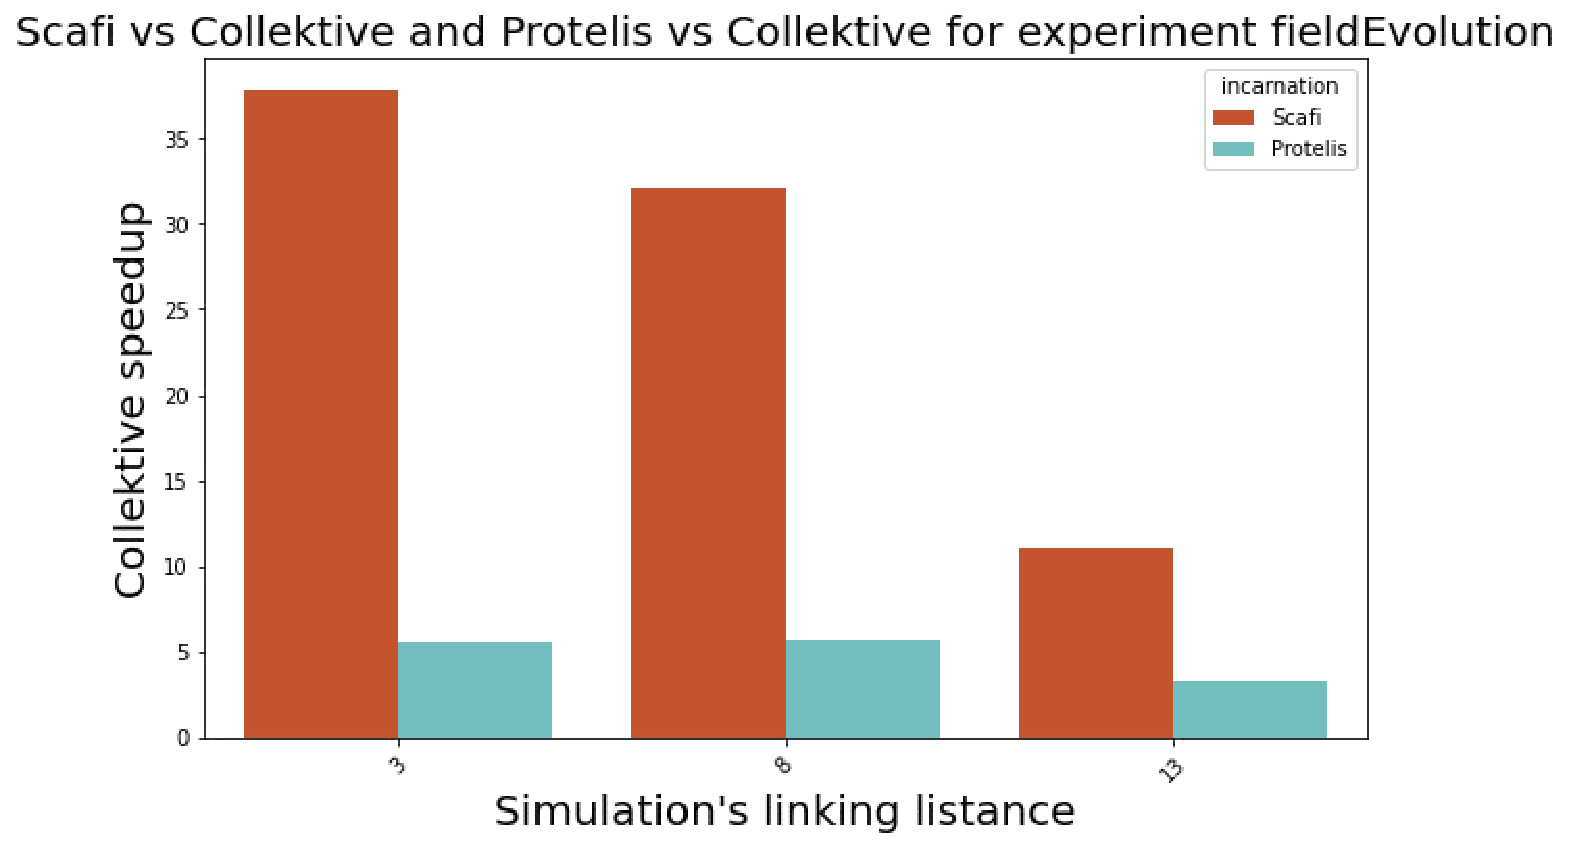
\includegraphics[width=\textwidth]{figures/field-speedup}
%    \end{subfigure}
    \begin{subfigure}[b]{0.49\textwidth}
        \centering
        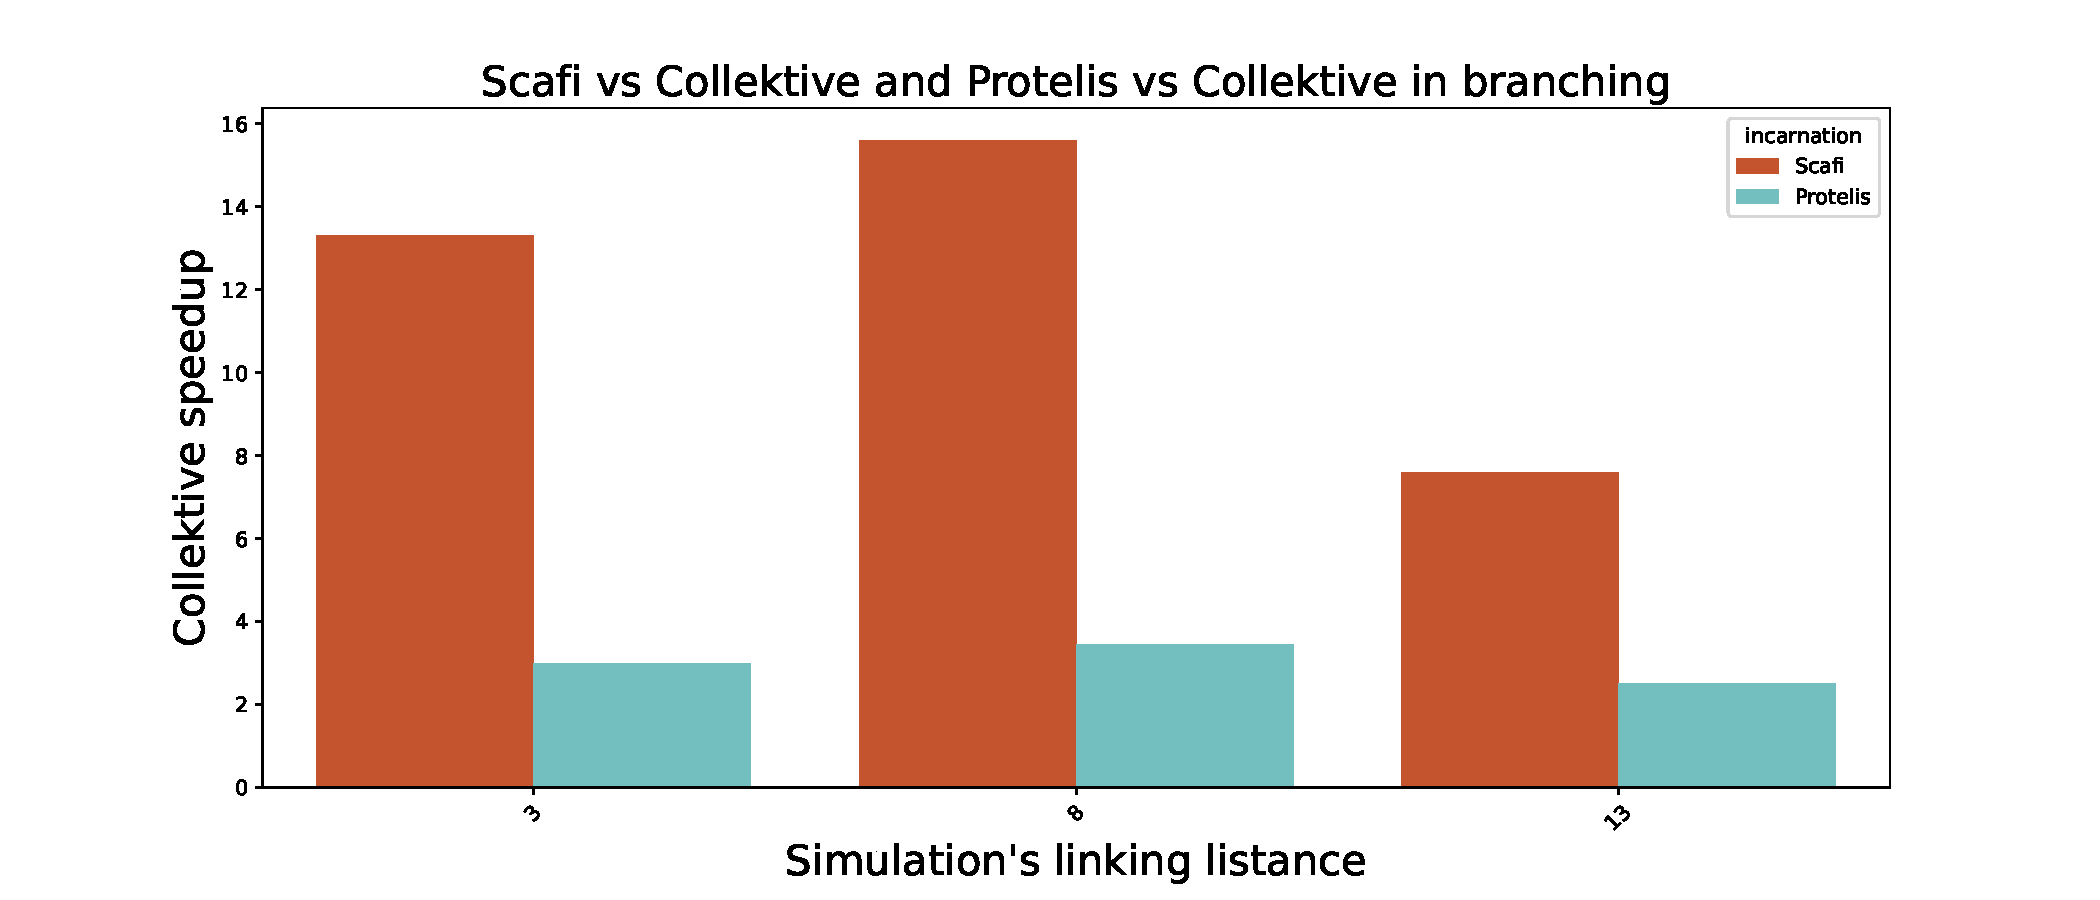
\includegraphics[width=\textwidth]{figures/branching-speedup}
    \end{subfigure}
    \begin{subfigure}[b]{0.49\textwidth}
        \centering
        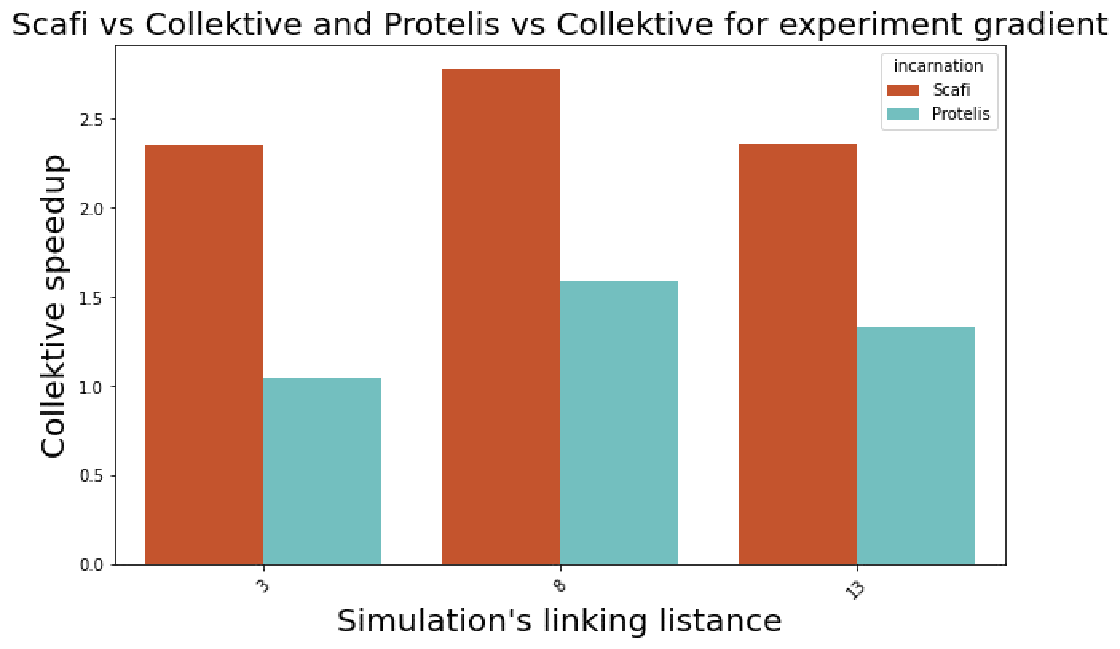
\includegraphics[width=\textwidth]{figures/gradient-speedup}
    \end{subfigure}
    \begin{subfigure}[b]{0.49\textwidth}
        \centering
        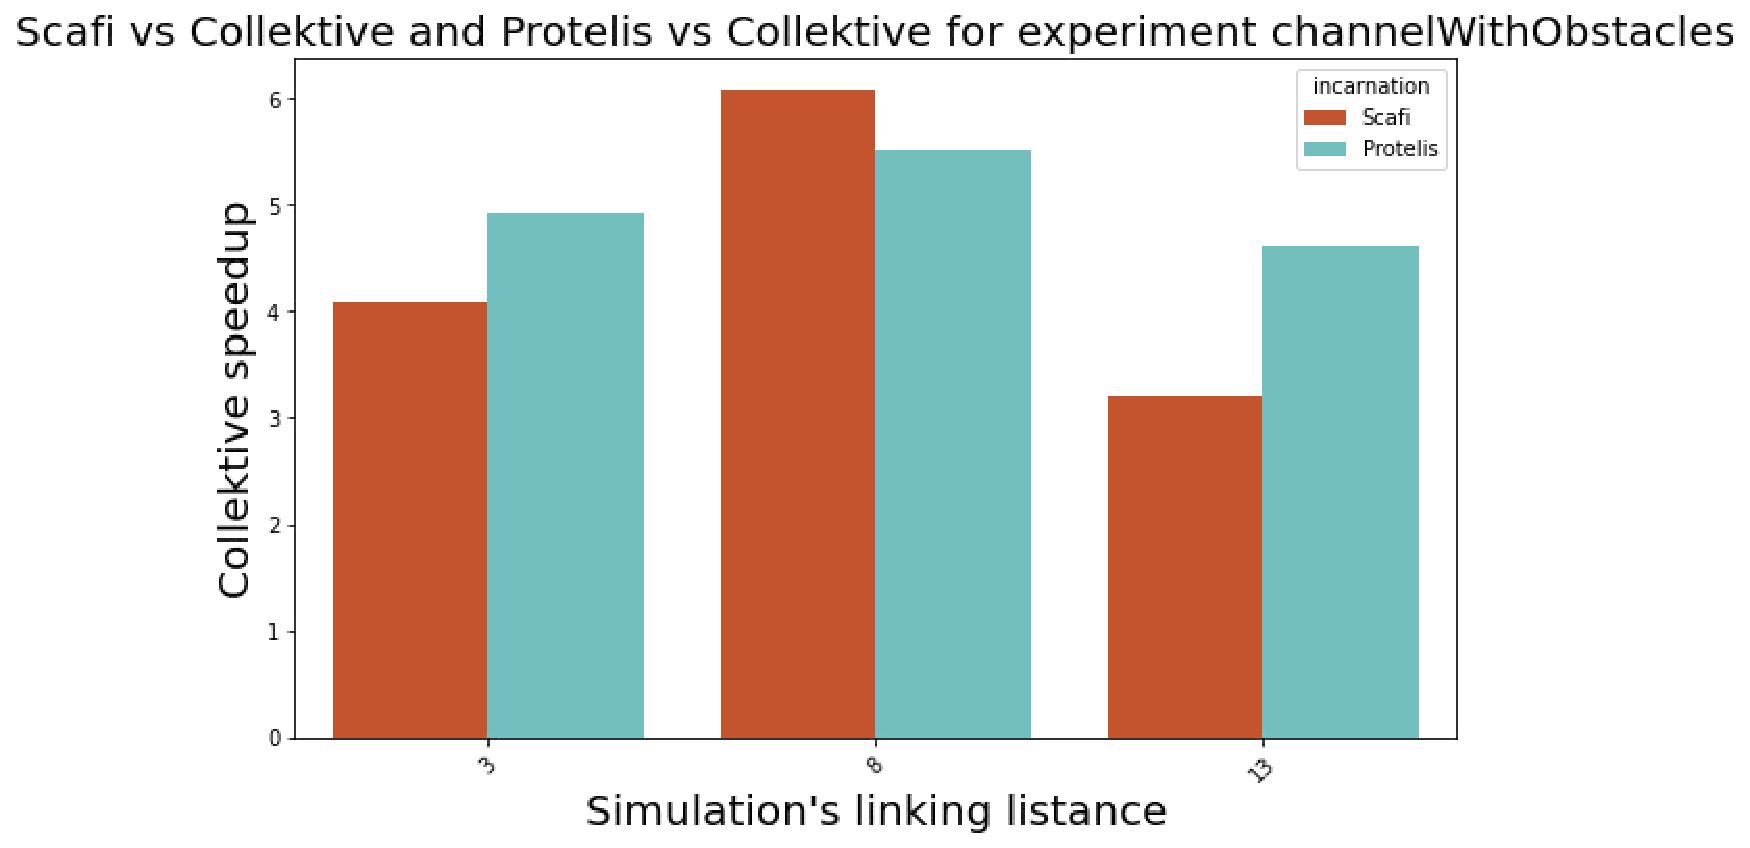
\includegraphics[width=\textwidth]{figures/channel-speedup}
    \end{subfigure}
    \caption{The speedup of the different incarnations with different network densities on the different tests.
        The speedup is calculated as the ratio between the average execution time of the other incarnations and the average
        execution time of \emph{Collektive}.}
    \label{fig:speedup}
\end{figure}

\paragraph{Conclusions}
Keeping in mind that the performance of the language may be influenced by the implementation of the incarnation, the results
show that \emph{Collektive} actually is faster than \emph{ScaFi} and \emph{Protelis} overall, with a significant
difference in the most complex programs, emphasizing the strength of \emph{Collektive} in managing fields and message exchanges.

For the easier tests, the difference is minimal between \emph{Collektive} and \emph{Protelis}, while it is significant
between \emph{Collektive} and \emph{ScaFi}.
With the growth in complexity of the tests, and in the density of the network, the difference between \emph{Collektive}
and the other languages becomes higher, showing the strength of the combination of \emph{Collektive}'s \ac{dsl} and its incarnation.

